\chapter{\iftoggle{german}{Konzept}{Concept}}\label{ch:concept}

In this chapter, we discuss the critical datasets used to create a new synthetic dataset and the reason for their selection.
Furthermore, how we combine multiple datasets to our advantage of creating new datasets in the Ersatz environment.
The rationale in choosing Unity as a framework to build the pipeline \autoref{sec:unity-based-pipeline}.
We will also discuss domain randomization  \autoref{subsec:domain-randomisation-with-unity-engine} and each of its parameters.
In \autoref{sec:s2r:3d-free-a-pix3d-based-synthetic-dataset}, we will introduce the proposed \gls{free} dataset used for the 3D-reconstruction task.

In the Deep Learning domain(\autoref{sec:3D reconstruction}), we explore what 3D-reconstruction is and how to achieve it.
In \autoref{subsec:pix2vox-and-pix2vox++}, the state-of-the-art models for 3D-Reconstruction on voxel representation and reason for selecting the sibling models as baselines are discussed.

\section{Pix3D: A large-scale benchmark}\label{sec:pix3d}
~\cite{pix3d}introduces a large-scale benchmark for 2D-3D alignment.
The raw images from web search engines were collected, and labeled key points were used to align the 2D images with the corresponding 3D shapes.
The 3D models extend the IKEA dataset~\cite{Lim2013ParsingIO}, a collection of high-quality IKEA furniture.
The dataset also provides a binary mask and the key points for the object under observation.
To add more images to the IKEA dataset, the authors of~\cite{pix3d} conducted a manual web search on Google, Bing, and Baidu, using the IKEA model name as keywords.
This search led to around 104,220 images which were further filtered by removing irrelevant images with the help of Amazon Mechanical Turk (AMT) workers.
After this manual experiment, the total images in Pix3D, only 14,600 images were selected for the 219 Ikea models.
For our synthetic to real dataset experiment, we chose to select only furniture classes from Pix3D, leaving out \”misc and tools\” classes, which were significantly less in comparison.


\subsection{Disadvantages of Pix3D}\label{subsec:disadvantages-of-pix3d}

The distribution of models in Pix3D is as shown in \autoref{fig:pix3d_histogram}.
As we can see, the dataset distribution is uneven across classes, and more than 50\% of classes have less than 1000 images.

Though Pix3D set a benchmark for 2D-3D alignment, here are few disadvantages of using this real dataset.
\begin{enumerate}
    \item For Deep Learning approaches, we need large-scale data, and 14,600 might not be sufficient.
    \item The orientation of an object is not randomized.
    \item The dataset does not provide 2.5D information (i.e., depth maps and normals), which can be crucial for 3D learning.
\end{enumerate}

\begin{figure}[!ht]
    \resizebox{0.49\textwidth}{6cm}{%% Creator: Matplotlib, PGF backend
%%
%% To include the figure in your LaTeX document, write
%%   \input{<filename>.pgf}
%%
%% Make sure the required packages are loaded in your preamble
%%   \usepackage{pgf}
%%
%% Figures using additional raster images can only be included by \input if
%% they are in the same directory as the main LaTeX file. For loading figures
%% from other directories you can use the `import` package
%%   \usepackage{import}
%%
%% and then include the figures with
%%   \import{<path to file>}{<filename>.pgf}
%%
%% Matplotlib used the following preamble
%%   \usepackage{fontspec}
%%   \setmainfont{DejaVuSerif.ttf}[Path=\detokenize{/Users/apple/opt/anaconda3/envs/kaolin/lib/python3.7/site-packages/matplotlib/mpl-data/fonts/ttf/}]
%%   \setsansfont{DejaVuSans.ttf}[Path=\detokenize{/Users/apple/opt/anaconda3/envs/kaolin/lib/python3.7/site-packages/matplotlib/mpl-data/fonts/ttf/}]
%%   \setmonofont{DejaVuSansMono.ttf}[Path=\detokenize{/Users/apple/opt/anaconda3/envs/kaolin/lib/python3.7/site-packages/matplotlib/mpl-data/fonts/ttf/}]
%%
\begingroup%
\makeatletter%
\begin{pgfpicture}%
\pgfpathrectangle{\pgfpointorigin}{\pgfqpoint{5.752068in}{4.226888in}}%
\pgfusepath{use as bounding box, clip}%
\begin{pgfscope}%
\pgfsetbuttcap%
\pgfsetmiterjoin%
\definecolor{currentfill}{rgb}{1.000000,1.000000,1.000000}%
\pgfsetfillcolor{currentfill}%
\pgfsetlinewidth{0.000000pt}%
\definecolor{currentstroke}{rgb}{1.000000,1.000000,1.000000}%
\pgfsetstrokecolor{currentstroke}%
\pgfsetdash{}{0pt}%
\pgfpathmoveto{\pgfqpoint{0.000000in}{0.000000in}}%
\pgfpathlineto{\pgfqpoint{5.752068in}{0.000000in}}%
\pgfpathlineto{\pgfqpoint{5.752068in}{4.226888in}}%
\pgfpathlineto{\pgfqpoint{0.000000in}{4.226888in}}%
\pgfpathclose%
\pgfusepath{fill}%
\end{pgfscope}%
\begin{pgfscope}%
\pgfsetbuttcap%
\pgfsetmiterjoin%
\definecolor{currentfill}{rgb}{1.000000,1.000000,1.000000}%
\pgfsetfillcolor{currentfill}%
\pgfsetlinewidth{0.000000pt}%
\definecolor{currentstroke}{rgb}{0.000000,0.000000,0.000000}%
\pgfsetstrokecolor{currentstroke}%
\pgfsetstrokeopacity{0.000000}%
\pgfsetdash{}{0pt}%
\pgfpathmoveto{\pgfqpoint{0.692068in}{0.385400in}}%
\pgfpathlineto{\pgfqpoint{5.652068in}{0.385400in}}%
\pgfpathlineto{\pgfqpoint{5.652068in}{4.081400in}}%
\pgfpathlineto{\pgfqpoint{0.692068in}{4.081400in}}%
\pgfpathclose%
\pgfusepath{fill}%
\end{pgfscope}%
\begin{pgfscope}%
\pgfpathrectangle{\pgfqpoint{0.692068in}{0.385400in}}{\pgfqpoint{4.960000in}{3.696000in}}%
\pgfusepath{clip}%
\pgfsetbuttcap%
\pgfsetmiterjoin%
\definecolor{currentfill}{rgb}{0.121569,0.466667,0.705882}%
\pgfsetfillcolor{currentfill}%
\pgfsetlinewidth{0.000000pt}%
\definecolor{currentstroke}{rgb}{0.000000,0.000000,0.000000}%
\pgfsetstrokecolor{currentstroke}%
\pgfsetstrokeopacity{0.000000}%
\pgfsetdash{}{0pt}%
\pgfpathmoveto{\pgfqpoint{0.917523in}{0.385400in}}%
\pgfpathlineto{\pgfqpoint{1.448004in}{0.385400in}}%
\pgfpathlineto{\pgfqpoint{1.448004in}{0.608208in}}%
\pgfpathlineto{\pgfqpoint{0.917523in}{0.608208in}}%
\pgfpathclose%
\pgfusepath{fill}%
\end{pgfscope}%
\begin{pgfscope}%
\pgfpathrectangle{\pgfqpoint{0.692068in}{0.385400in}}{\pgfqpoint{4.960000in}{3.696000in}}%
\pgfusepath{clip}%
\pgfsetbuttcap%
\pgfsetmiterjoin%
\definecolor{currentfill}{rgb}{0.121569,0.466667,0.705882}%
\pgfsetfillcolor{currentfill}%
\pgfsetlinewidth{0.000000pt}%
\definecolor{currentstroke}{rgb}{0.000000,0.000000,0.000000}%
\pgfsetstrokecolor{currentstroke}%
\pgfsetstrokeopacity{0.000000}%
\pgfsetdash{}{0pt}%
\pgfpathmoveto{\pgfqpoint{1.580624in}{0.385400in}}%
\pgfpathlineto{\pgfqpoint{2.111105in}{0.385400in}}%
\pgfpathlineto{\pgfqpoint{2.111105in}{1.296804in}}%
\pgfpathlineto{\pgfqpoint{1.580624in}{1.296804in}}%
\pgfpathclose%
\pgfusepath{fill}%
\end{pgfscope}%
\begin{pgfscope}%
\pgfpathrectangle{\pgfqpoint{0.692068in}{0.385400in}}{\pgfqpoint{4.960000in}{3.696000in}}%
\pgfusepath{clip}%
\pgfsetbuttcap%
\pgfsetmiterjoin%
\definecolor{currentfill}{rgb}{0.121569,0.466667,0.705882}%
\pgfsetfillcolor{currentfill}%
\pgfsetlinewidth{0.000000pt}%
\definecolor{currentstroke}{rgb}{0.000000,0.000000,0.000000}%
\pgfsetstrokecolor{currentstroke}%
\pgfsetstrokeopacity{0.000000}%
\pgfsetdash{}{0pt}%
\pgfpathmoveto{\pgfqpoint{2.243726in}{0.385400in}}%
\pgfpathlineto{\pgfqpoint{2.774207in}{0.385400in}}%
\pgfpathlineto{\pgfqpoint{2.774207in}{1.028151in}}%
\pgfpathlineto{\pgfqpoint{2.243726in}{1.028151in}}%
\pgfpathclose%
\pgfusepath{fill}%
\end{pgfscope}%
\begin{pgfscope}%
\pgfpathrectangle{\pgfqpoint{0.692068in}{0.385400in}}{\pgfqpoint{4.960000in}{3.696000in}}%
\pgfusepath{clip}%
\pgfsetbuttcap%
\pgfsetmiterjoin%
\definecolor{currentfill}{rgb}{0.121569,0.466667,0.705882}%
\pgfsetfillcolor{currentfill}%
\pgfsetlinewidth{0.000000pt}%
\definecolor{currentstroke}{rgb}{0.000000,0.000000,0.000000}%
\pgfsetstrokecolor{currentstroke}%
\pgfsetstrokeopacity{0.000000}%
\pgfsetdash{}{0pt}%
\pgfpathmoveto{\pgfqpoint{2.906827in}{0.385400in}}%
\pgfpathlineto{\pgfqpoint{3.437309in}{0.385400in}}%
\pgfpathlineto{\pgfqpoint{3.437309in}{3.905400in}}%
\pgfpathlineto{\pgfqpoint{2.906827in}{3.905400in}}%
\pgfpathclose%
\pgfusepath{fill}%
\end{pgfscope}%
\begin{pgfscope}%
\pgfpathrectangle{\pgfqpoint{0.692068in}{0.385400in}}{\pgfqpoint{4.960000in}{3.696000in}}%
\pgfusepath{clip}%
\pgfsetbuttcap%
\pgfsetmiterjoin%
\definecolor{currentfill}{rgb}{0.121569,0.466667,0.705882}%
\pgfsetfillcolor{currentfill}%
\pgfsetlinewidth{0.000000pt}%
\definecolor{currentstroke}{rgb}{0.000000,0.000000,0.000000}%
\pgfsetstrokecolor{currentstroke}%
\pgfsetstrokeopacity{0.000000}%
\pgfsetdash{}{0pt}%
\pgfpathmoveto{\pgfqpoint{3.569929in}{0.385400in}}%
\pgfpathlineto{\pgfqpoint{4.100410in}{0.385400in}}%
\pgfpathlineto{\pgfqpoint{4.100410in}{0.716403in}}%
\pgfpathlineto{\pgfqpoint{3.569929in}{0.716403in}}%
\pgfpathclose%
\pgfusepath{fill}%
\end{pgfscope}%
\begin{pgfscope}%
\pgfpathrectangle{\pgfqpoint{0.692068in}{0.385400in}}{\pgfqpoint{4.960000in}{3.696000in}}%
\pgfusepath{clip}%
\pgfsetbuttcap%
\pgfsetmiterjoin%
\definecolor{currentfill}{rgb}{0.121569,0.466667,0.705882}%
\pgfsetfillcolor{currentfill}%
\pgfsetlinewidth{0.000000pt}%
\definecolor{currentstroke}{rgb}{0.000000,0.000000,0.000000}%
\pgfsetstrokecolor{currentstroke}%
\pgfsetstrokeopacity{0.000000}%
\pgfsetdash{}{0pt}%
\pgfpathmoveto{\pgfqpoint{4.233031in}{0.385400in}}%
\pgfpathlineto{\pgfqpoint{4.763512in}{0.385400in}}%
\pgfpathlineto{\pgfqpoint{4.763512in}{2.171532in}}%
\pgfpathlineto{\pgfqpoint{4.233031in}{2.171532in}}%
\pgfpathclose%
\pgfusepath{fill}%
\end{pgfscope}%
\begin{pgfscope}%
\pgfpathrectangle{\pgfqpoint{0.692068in}{0.385400in}}{\pgfqpoint{4.960000in}{3.696000in}}%
\pgfusepath{clip}%
\pgfsetbuttcap%
\pgfsetmiterjoin%
\definecolor{currentfill}{rgb}{0.121569,0.466667,0.705882}%
\pgfsetfillcolor{currentfill}%
\pgfsetlinewidth{0.000000pt}%
\definecolor{currentstroke}{rgb}{0.000000,0.000000,0.000000}%
\pgfsetstrokecolor{currentstroke}%
\pgfsetstrokeopacity{0.000000}%
\pgfsetdash{}{0pt}%
\pgfpathmoveto{\pgfqpoint{4.896132in}{0.385400in}}%
\pgfpathlineto{\pgfqpoint{5.426614in}{0.385400in}}%
\pgfpathlineto{\pgfqpoint{5.426614in}{2.100013in}}%
\pgfpathlineto{\pgfqpoint{4.896132in}{2.100013in}}%
\pgfpathclose%
\pgfusepath{fill}%
\end{pgfscope}%
\begin{pgfscope}%
\pgfsetbuttcap%
\pgfsetroundjoin%
\definecolor{currentfill}{rgb}{0.000000,0.000000,0.000000}%
\pgfsetfillcolor{currentfill}%
\pgfsetlinewidth{0.803000pt}%
\definecolor{currentstroke}{rgb}{0.000000,0.000000,0.000000}%
\pgfsetstrokecolor{currentstroke}%
\pgfsetdash{}{0pt}%
\pgfsys@defobject{currentmarker}{\pgfqpoint{0.000000in}{-0.048611in}}{\pgfqpoint{0.000000in}{0.000000in}}{%
\pgfpathmoveto{\pgfqpoint{0.000000in}{0.000000in}}%
\pgfpathlineto{\pgfqpoint{0.000000in}{-0.048611in}}%
\pgfusepath{stroke,fill}%
}%
\begin{pgfscope}%
\pgfsys@transformshift{1.182763in}{0.385400in}%
\pgfsys@useobject{currentmarker}{}%
\end{pgfscope}%
\end{pgfscope}%
\begin{pgfscope}%
\definecolor{textcolor}{rgb}{0.000000,0.000000,0.000000}%
\pgfsetstrokecolor{textcolor}%
\pgfsetfillcolor{textcolor}%
\pgftext[x=1.182763in,y=0.288178in,,top]{\color{textcolor}\sffamily\fontsize{14.000000}{16.800000}\selectfont wardrobe}%
\end{pgfscope}%
\begin{pgfscope}%
\pgfsetbuttcap%
\pgfsetroundjoin%
\definecolor{currentfill}{rgb}{0.000000,0.000000,0.000000}%
\pgfsetfillcolor{currentfill}%
\pgfsetlinewidth{0.803000pt}%
\definecolor{currentstroke}{rgb}{0.000000,0.000000,0.000000}%
\pgfsetstrokecolor{currentstroke}%
\pgfsetdash{}{0pt}%
\pgfsys@defobject{currentmarker}{\pgfqpoint{0.000000in}{-0.048611in}}{\pgfqpoint{0.000000in}{0.000000in}}{%
\pgfpathmoveto{\pgfqpoint{0.000000in}{0.000000in}}%
\pgfpathlineto{\pgfqpoint{0.000000in}{-0.048611in}}%
\pgfusepath{stroke,fill}%
}%
\begin{pgfscope}%
\pgfsys@transformshift{1.845865in}{0.385400in}%
\pgfsys@useobject{currentmarker}{}%
\end{pgfscope}%
\end{pgfscope}%
\begin{pgfscope}%
\definecolor{textcolor}{rgb}{0.000000,0.000000,0.000000}%
\pgfsetstrokecolor{textcolor}%
\pgfsetfillcolor{textcolor}%
\pgftext[x=1.845865in,y=0.288178in,,top]{\color{textcolor}\sffamily\fontsize{14.000000}{16.800000}\selectfont bed}%
\end{pgfscope}%
\begin{pgfscope}%
\pgfsetbuttcap%
\pgfsetroundjoin%
\definecolor{currentfill}{rgb}{0.000000,0.000000,0.000000}%
\pgfsetfillcolor{currentfill}%
\pgfsetlinewidth{0.803000pt}%
\definecolor{currentstroke}{rgb}{0.000000,0.000000,0.000000}%
\pgfsetstrokecolor{currentstroke}%
\pgfsetdash{}{0pt}%
\pgfsys@defobject{currentmarker}{\pgfqpoint{0.000000in}{-0.048611in}}{\pgfqpoint{0.000000in}{0.000000in}}{%
\pgfpathmoveto{\pgfqpoint{0.000000in}{0.000000in}}%
\pgfpathlineto{\pgfqpoint{0.000000in}{-0.048611in}}%
\pgfusepath{stroke,fill}%
}%
\begin{pgfscope}%
\pgfsys@transformshift{2.508966in}{0.385400in}%
\pgfsys@useobject{currentmarker}{}%
\end{pgfscope}%
\end{pgfscope}%
\begin{pgfscope}%
\definecolor{textcolor}{rgb}{0.000000,0.000000,0.000000}%
\pgfsetstrokecolor{textcolor}%
\pgfsetfillcolor{textcolor}%
\pgftext[x=2.508966in,y=0.288178in,,top]{\color{textcolor}\sffamily\fontsize{14.000000}{16.800000}\selectfont desk}%
\end{pgfscope}%
\begin{pgfscope}%
\pgfsetbuttcap%
\pgfsetroundjoin%
\definecolor{currentfill}{rgb}{0.000000,0.000000,0.000000}%
\pgfsetfillcolor{currentfill}%
\pgfsetlinewidth{0.803000pt}%
\definecolor{currentstroke}{rgb}{0.000000,0.000000,0.000000}%
\pgfsetstrokecolor{currentstroke}%
\pgfsetdash{}{0pt}%
\pgfsys@defobject{currentmarker}{\pgfqpoint{0.000000in}{-0.048611in}}{\pgfqpoint{0.000000in}{0.000000in}}{%
\pgfpathmoveto{\pgfqpoint{0.000000in}{0.000000in}}%
\pgfpathlineto{\pgfqpoint{0.000000in}{-0.048611in}}%
\pgfusepath{stroke,fill}%
}%
\begin{pgfscope}%
\pgfsys@transformshift{3.172068in}{0.385400in}%
\pgfsys@useobject{currentmarker}{}%
\end{pgfscope}%
\end{pgfscope}%
\begin{pgfscope}%
\definecolor{textcolor}{rgb}{0.000000,0.000000,0.000000}%
\pgfsetstrokecolor{textcolor}%
\pgfsetfillcolor{textcolor}%
\pgftext[x=3.172068in,y=0.288178in,,top]{\color{textcolor}\sffamily\fontsize{14.000000}{16.800000}\selectfont chair}%
\end{pgfscope}%
\begin{pgfscope}%
\pgfsetbuttcap%
\pgfsetroundjoin%
\definecolor{currentfill}{rgb}{0.000000,0.000000,0.000000}%
\pgfsetfillcolor{currentfill}%
\pgfsetlinewidth{0.803000pt}%
\definecolor{currentstroke}{rgb}{0.000000,0.000000,0.000000}%
\pgfsetstrokecolor{currentstroke}%
\pgfsetdash{}{0pt}%
\pgfsys@defobject{currentmarker}{\pgfqpoint{0.000000in}{-0.048611in}}{\pgfqpoint{0.000000in}{0.000000in}}{%
\pgfpathmoveto{\pgfqpoint{0.000000in}{0.000000in}}%
\pgfpathlineto{\pgfqpoint{0.000000in}{-0.048611in}}%
\pgfusepath{stroke,fill}%
}%
\begin{pgfscope}%
\pgfsys@transformshift{3.835170in}{0.385400in}%
\pgfsys@useobject{currentmarker}{}%
\end{pgfscope}%
\end{pgfscope}%
\begin{pgfscope}%
\definecolor{textcolor}{rgb}{0.000000,0.000000,0.000000}%
\pgfsetstrokecolor{textcolor}%
\pgfsetfillcolor{textcolor}%
\pgftext[x=3.835170in,y=0.288178in,,top]{\color{textcolor}\sffamily\fontsize{14.000000}{16.800000}\selectfont bookcase}%
\end{pgfscope}%
\begin{pgfscope}%
\pgfsetbuttcap%
\pgfsetroundjoin%
\definecolor{currentfill}{rgb}{0.000000,0.000000,0.000000}%
\pgfsetfillcolor{currentfill}%
\pgfsetlinewidth{0.803000pt}%
\definecolor{currentstroke}{rgb}{0.000000,0.000000,0.000000}%
\pgfsetstrokecolor{currentstroke}%
\pgfsetdash{}{0pt}%
\pgfsys@defobject{currentmarker}{\pgfqpoint{0.000000in}{-0.048611in}}{\pgfqpoint{0.000000in}{0.000000in}}{%
\pgfpathmoveto{\pgfqpoint{0.000000in}{0.000000in}}%
\pgfpathlineto{\pgfqpoint{0.000000in}{-0.048611in}}%
\pgfusepath{stroke,fill}%
}%
\begin{pgfscope}%
\pgfsys@transformshift{4.498271in}{0.385400in}%
\pgfsys@useobject{currentmarker}{}%
\end{pgfscope}%
\end{pgfscope}%
\begin{pgfscope}%
\definecolor{textcolor}{rgb}{0.000000,0.000000,0.000000}%
\pgfsetstrokecolor{textcolor}%
\pgfsetfillcolor{textcolor}%
\pgftext[x=4.498271in,y=0.288178in,,top]{\color{textcolor}\sffamily\fontsize{14.000000}{16.800000}\selectfont sofa}%
\end{pgfscope}%
\begin{pgfscope}%
\pgfsetbuttcap%
\pgfsetroundjoin%
\definecolor{currentfill}{rgb}{0.000000,0.000000,0.000000}%
\pgfsetfillcolor{currentfill}%
\pgfsetlinewidth{0.803000pt}%
\definecolor{currentstroke}{rgb}{0.000000,0.000000,0.000000}%
\pgfsetstrokecolor{currentstroke}%
\pgfsetdash{}{0pt}%
\pgfsys@defobject{currentmarker}{\pgfqpoint{0.000000in}{-0.048611in}}{\pgfqpoint{0.000000in}{0.000000in}}{%
\pgfpathmoveto{\pgfqpoint{0.000000in}{0.000000in}}%
\pgfpathlineto{\pgfqpoint{0.000000in}{-0.048611in}}%
\pgfusepath{stroke,fill}%
}%
\begin{pgfscope}%
\pgfsys@transformshift{5.161373in}{0.385400in}%
\pgfsys@useobject{currentmarker}{}%
\end{pgfscope}%
\end{pgfscope}%
\begin{pgfscope}%
\definecolor{textcolor}{rgb}{0.000000,0.000000,0.000000}%
\pgfsetstrokecolor{textcolor}%
\pgfsetfillcolor{textcolor}%
\pgftext[x=5.161373in,y=0.288178in,,top]{\color{textcolor}\sffamily\fontsize{14.000000}{16.800000}\selectfont table}%
\end{pgfscope}%
\begin{pgfscope}%
\pgfsetbuttcap%
\pgfsetroundjoin%
\definecolor{currentfill}{rgb}{0.000000,0.000000,0.000000}%
\pgfsetfillcolor{currentfill}%
\pgfsetlinewidth{0.803000pt}%
\definecolor{currentstroke}{rgb}{0.000000,0.000000,0.000000}%
\pgfsetstrokecolor{currentstroke}%
\pgfsetdash{}{0pt}%
\pgfsys@defobject{currentmarker}{\pgfqpoint{-0.048611in}{0.000000in}}{\pgfqpoint{-0.000000in}{0.000000in}}{%
\pgfpathmoveto{\pgfqpoint{-0.000000in}{0.000000in}}%
\pgfpathlineto{\pgfqpoint{-0.048611in}{0.000000in}}%
\pgfusepath{stroke,fill}%
}%
\begin{pgfscope}%
\pgfsys@transformshift{0.692068in}{0.385400in}%
\pgfsys@useobject{currentmarker}{}%
\end{pgfscope}%
\end{pgfscope}%
\begin{pgfscope}%
\definecolor{textcolor}{rgb}{0.000000,0.000000,0.000000}%
\pgfsetstrokecolor{textcolor}%
\pgfsetfillcolor{textcolor}%
\pgftext[x=0.471134in, y=0.311534in, left, base]{\color{textcolor}\sffamily\fontsize{14.000000}{16.800000}\selectfont 0}%
\end{pgfscope}%
\begin{pgfscope}%
\pgfsetbuttcap%
\pgfsetroundjoin%
\definecolor{currentfill}{rgb}{0.000000,0.000000,0.000000}%
\pgfsetfillcolor{currentfill}%
\pgfsetlinewidth{0.803000pt}%
\definecolor{currentstroke}{rgb}{0.000000,0.000000,0.000000}%
\pgfsetstrokecolor{currentstroke}%
\pgfsetdash{}{0pt}%
\pgfsys@defobject{currentmarker}{\pgfqpoint{-0.048611in}{0.000000in}}{\pgfqpoint{-0.000000in}{0.000000in}}{%
\pgfpathmoveto{\pgfqpoint{-0.000000in}{0.000000in}}%
\pgfpathlineto{\pgfqpoint{-0.048611in}{0.000000in}}%
\pgfusepath{stroke,fill}%
}%
\begin{pgfscope}%
\pgfsys@transformshift{0.692068in}{0.843853in}%
\pgfsys@useobject{currentmarker}{}%
\end{pgfscope}%
\end{pgfscope}%
\begin{pgfscope}%
\definecolor{textcolor}{rgb}{0.000000,0.000000,0.000000}%
\pgfsetstrokecolor{textcolor}%
\pgfsetfillcolor{textcolor}%
\pgftext[x=0.223711in, y=0.769987in, left, base]{\color{textcolor}\sffamily\fontsize{14.000000}{16.800000}\selectfont 500}%
\end{pgfscope}%
\begin{pgfscope}%
\pgfsetbuttcap%
\pgfsetroundjoin%
\definecolor{currentfill}{rgb}{0.000000,0.000000,0.000000}%
\pgfsetfillcolor{currentfill}%
\pgfsetlinewidth{0.803000pt}%
\definecolor{currentstroke}{rgb}{0.000000,0.000000,0.000000}%
\pgfsetstrokecolor{currentstroke}%
\pgfsetdash{}{0pt}%
\pgfsys@defobject{currentmarker}{\pgfqpoint{-0.048611in}{0.000000in}}{\pgfqpoint{-0.000000in}{0.000000in}}{%
\pgfpathmoveto{\pgfqpoint{-0.000000in}{0.000000in}}%
\pgfpathlineto{\pgfqpoint{-0.048611in}{0.000000in}}%
\pgfusepath{stroke,fill}%
}%
\begin{pgfscope}%
\pgfsys@transformshift{0.692068in}{1.302306in}%
\pgfsys@useobject{currentmarker}{}%
\end{pgfscope}%
\end{pgfscope}%
\begin{pgfscope}%
\definecolor{textcolor}{rgb}{0.000000,0.000000,0.000000}%
\pgfsetstrokecolor{textcolor}%
\pgfsetfillcolor{textcolor}%
\pgftext[x=0.100000in, y=1.228440in, left, base]{\color{textcolor}\sffamily\fontsize{14.000000}{16.800000}\selectfont 1000}%
\end{pgfscope}%
\begin{pgfscope}%
\pgfsetbuttcap%
\pgfsetroundjoin%
\definecolor{currentfill}{rgb}{0.000000,0.000000,0.000000}%
\pgfsetfillcolor{currentfill}%
\pgfsetlinewidth{0.803000pt}%
\definecolor{currentstroke}{rgb}{0.000000,0.000000,0.000000}%
\pgfsetstrokecolor{currentstroke}%
\pgfsetdash{}{0pt}%
\pgfsys@defobject{currentmarker}{\pgfqpoint{-0.048611in}{0.000000in}}{\pgfqpoint{-0.000000in}{0.000000in}}{%
\pgfpathmoveto{\pgfqpoint{-0.000000in}{0.000000in}}%
\pgfpathlineto{\pgfqpoint{-0.048611in}{0.000000in}}%
\pgfusepath{stroke,fill}%
}%
\begin{pgfscope}%
\pgfsys@transformshift{0.692068in}{1.760758in}%
\pgfsys@useobject{currentmarker}{}%
\end{pgfscope}%
\end{pgfscope}%
\begin{pgfscope}%
\definecolor{textcolor}{rgb}{0.000000,0.000000,0.000000}%
\pgfsetstrokecolor{textcolor}%
\pgfsetfillcolor{textcolor}%
\pgftext[x=0.100000in, y=1.686892in, left, base]{\color{textcolor}\sffamily\fontsize{14.000000}{16.800000}\selectfont 1500}%
\end{pgfscope}%
\begin{pgfscope}%
\pgfsetbuttcap%
\pgfsetroundjoin%
\definecolor{currentfill}{rgb}{0.000000,0.000000,0.000000}%
\pgfsetfillcolor{currentfill}%
\pgfsetlinewidth{0.803000pt}%
\definecolor{currentstroke}{rgb}{0.000000,0.000000,0.000000}%
\pgfsetstrokecolor{currentstroke}%
\pgfsetdash{}{0pt}%
\pgfsys@defobject{currentmarker}{\pgfqpoint{-0.048611in}{0.000000in}}{\pgfqpoint{-0.000000in}{0.000000in}}{%
\pgfpathmoveto{\pgfqpoint{-0.000000in}{0.000000in}}%
\pgfpathlineto{\pgfqpoint{-0.048611in}{0.000000in}}%
\pgfusepath{stroke,fill}%
}%
\begin{pgfscope}%
\pgfsys@transformshift{0.692068in}{2.219211in}%
\pgfsys@useobject{currentmarker}{}%
\end{pgfscope}%
\end{pgfscope}%
\begin{pgfscope}%
\definecolor{textcolor}{rgb}{0.000000,0.000000,0.000000}%
\pgfsetstrokecolor{textcolor}%
\pgfsetfillcolor{textcolor}%
\pgftext[x=0.100000in, y=2.145345in, left, base]{\color{textcolor}\sffamily\fontsize{14.000000}{16.800000}\selectfont 2000}%
\end{pgfscope}%
\begin{pgfscope}%
\pgfsetbuttcap%
\pgfsetroundjoin%
\definecolor{currentfill}{rgb}{0.000000,0.000000,0.000000}%
\pgfsetfillcolor{currentfill}%
\pgfsetlinewidth{0.803000pt}%
\definecolor{currentstroke}{rgb}{0.000000,0.000000,0.000000}%
\pgfsetstrokecolor{currentstroke}%
\pgfsetdash{}{0pt}%
\pgfsys@defobject{currentmarker}{\pgfqpoint{-0.048611in}{0.000000in}}{\pgfqpoint{-0.000000in}{0.000000in}}{%
\pgfpathmoveto{\pgfqpoint{-0.000000in}{0.000000in}}%
\pgfpathlineto{\pgfqpoint{-0.048611in}{0.000000in}}%
\pgfusepath{stroke,fill}%
}%
\begin{pgfscope}%
\pgfsys@transformshift{0.692068in}{2.677664in}%
\pgfsys@useobject{currentmarker}{}%
\end{pgfscope}%
\end{pgfscope}%
\begin{pgfscope}%
\definecolor{textcolor}{rgb}{0.000000,0.000000,0.000000}%
\pgfsetstrokecolor{textcolor}%
\pgfsetfillcolor{textcolor}%
\pgftext[x=0.100000in, y=2.603798in, left, base]{\color{textcolor}\sffamily\fontsize{14.000000}{16.800000}\selectfont 2500}%
\end{pgfscope}%
\begin{pgfscope}%
\pgfsetbuttcap%
\pgfsetroundjoin%
\definecolor{currentfill}{rgb}{0.000000,0.000000,0.000000}%
\pgfsetfillcolor{currentfill}%
\pgfsetlinewidth{0.803000pt}%
\definecolor{currentstroke}{rgb}{0.000000,0.000000,0.000000}%
\pgfsetstrokecolor{currentstroke}%
\pgfsetdash{}{0pt}%
\pgfsys@defobject{currentmarker}{\pgfqpoint{-0.048611in}{0.000000in}}{\pgfqpoint{-0.000000in}{0.000000in}}{%
\pgfpathmoveto{\pgfqpoint{-0.000000in}{0.000000in}}%
\pgfpathlineto{\pgfqpoint{-0.048611in}{0.000000in}}%
\pgfusepath{stroke,fill}%
}%
\begin{pgfscope}%
\pgfsys@transformshift{0.692068in}{3.136117in}%
\pgfsys@useobject{currentmarker}{}%
\end{pgfscope}%
\end{pgfscope}%
\begin{pgfscope}%
\definecolor{textcolor}{rgb}{0.000000,0.000000,0.000000}%
\pgfsetstrokecolor{textcolor}%
\pgfsetfillcolor{textcolor}%
\pgftext[x=0.100000in, y=3.062250in, left, base]{\color{textcolor}\sffamily\fontsize{14.000000}{16.800000}\selectfont 3000}%
\end{pgfscope}%
\begin{pgfscope}%
\pgfsetbuttcap%
\pgfsetroundjoin%
\definecolor{currentfill}{rgb}{0.000000,0.000000,0.000000}%
\pgfsetfillcolor{currentfill}%
\pgfsetlinewidth{0.803000pt}%
\definecolor{currentstroke}{rgb}{0.000000,0.000000,0.000000}%
\pgfsetstrokecolor{currentstroke}%
\pgfsetdash{}{0pt}%
\pgfsys@defobject{currentmarker}{\pgfqpoint{-0.048611in}{0.000000in}}{\pgfqpoint{-0.000000in}{0.000000in}}{%
\pgfpathmoveto{\pgfqpoint{-0.000000in}{0.000000in}}%
\pgfpathlineto{\pgfqpoint{-0.048611in}{0.000000in}}%
\pgfusepath{stroke,fill}%
}%
\begin{pgfscope}%
\pgfsys@transformshift{0.692068in}{3.594569in}%
\pgfsys@useobject{currentmarker}{}%
\end{pgfscope}%
\end{pgfscope}%
\begin{pgfscope}%
\definecolor{textcolor}{rgb}{0.000000,0.000000,0.000000}%
\pgfsetstrokecolor{textcolor}%
\pgfsetfillcolor{textcolor}%
\pgftext[x=0.100000in, y=3.520703in, left, base]{\color{textcolor}\sffamily\fontsize{14.000000}{16.800000}\selectfont 3500}%
\end{pgfscope}%
\begin{pgfscope}%
\pgfsetbuttcap%
\pgfsetroundjoin%
\definecolor{currentfill}{rgb}{0.000000,0.000000,0.000000}%
\pgfsetfillcolor{currentfill}%
\pgfsetlinewidth{0.803000pt}%
\definecolor{currentstroke}{rgb}{0.000000,0.000000,0.000000}%
\pgfsetstrokecolor{currentstroke}%
\pgfsetdash{}{0pt}%
\pgfsys@defobject{currentmarker}{\pgfqpoint{-0.048611in}{0.000000in}}{\pgfqpoint{-0.000000in}{0.000000in}}{%
\pgfpathmoveto{\pgfqpoint{-0.000000in}{0.000000in}}%
\pgfpathlineto{\pgfqpoint{-0.048611in}{0.000000in}}%
\pgfusepath{stroke,fill}%
}%
\begin{pgfscope}%
\pgfsys@transformshift{0.692068in}{4.053022in}%
\pgfsys@useobject{currentmarker}{}%
\end{pgfscope}%
\end{pgfscope}%
\begin{pgfscope}%
\definecolor{textcolor}{rgb}{0.000000,0.000000,0.000000}%
\pgfsetstrokecolor{textcolor}%
\pgfsetfillcolor{textcolor}%
\pgftext[x=0.100000in, y=3.979156in, left, base]{\color{textcolor}\sffamily\fontsize{14.000000}{16.800000}\selectfont 4000}%
\end{pgfscope}%
\begin{pgfscope}%
\pgfsetrectcap%
\pgfsetmiterjoin%
\pgfsetlinewidth{0.803000pt}%
\definecolor{currentstroke}{rgb}{0.000000,0.000000,0.000000}%
\pgfsetstrokecolor{currentstroke}%
\pgfsetdash{}{0pt}%
\pgfpathmoveto{\pgfqpoint{0.692068in}{0.385400in}}%
\pgfpathlineto{\pgfqpoint{0.692068in}{4.081400in}}%
\pgfusepath{stroke}%
\end{pgfscope}%
\begin{pgfscope}%
\pgfsetrectcap%
\pgfsetmiterjoin%
\pgfsetlinewidth{0.803000pt}%
\definecolor{currentstroke}{rgb}{0.000000,0.000000,0.000000}%
\pgfsetstrokecolor{currentstroke}%
\pgfsetdash{}{0pt}%
\pgfpathmoveto{\pgfqpoint{5.652068in}{0.385400in}}%
\pgfpathlineto{\pgfqpoint{5.652068in}{4.081400in}}%
\pgfusepath{stroke}%
\end{pgfscope}%
\begin{pgfscope}%
\pgfsetrectcap%
\pgfsetmiterjoin%
\pgfsetlinewidth{0.803000pt}%
\definecolor{currentstroke}{rgb}{0.000000,0.000000,0.000000}%
\pgfsetstrokecolor{currentstroke}%
\pgfsetdash{}{0pt}%
\pgfpathmoveto{\pgfqpoint{0.692068in}{0.385400in}}%
\pgfpathlineto{\pgfqpoint{5.652068in}{0.385400in}}%
\pgfusepath{stroke}%
\end{pgfscope}%
\begin{pgfscope}%
\pgfsetrectcap%
\pgfsetmiterjoin%
\pgfsetlinewidth{0.803000pt}%
\definecolor{currentstroke}{rgb}{0.000000,0.000000,0.000000}%
\pgfsetstrokecolor{currentstroke}%
\pgfsetdash{}{0pt}%
\pgfpathmoveto{\pgfqpoint{0.692068in}{4.081400in}}%
\pgfpathlineto{\pgfqpoint{5.652068in}{4.081400in}}%
\pgfusepath{stroke}%
\end{pgfscope}%
\end{pgfpicture}%
\makeatother%
\endgroup%
}
    \resizebox{0.49\textwidth}{6cm}{%% Creator: Matplotlib, PGF backend
%%
%% To include the figure in your LaTeX document, write
%%   \input{<filename>.pgf}
%%
%% Make sure the required packages are loaded in your preamble
%%   \usepackage{pgf}
%%
%% Figures using additional raster images can only be included by \input if
%% they are in the same directory as the main LaTeX file. For loading figures
%% from other directories you can use the `import` package
%%   \usepackage{import}
%%
%% and then include the figures with
%%   \import{<path to file>}{<filename>.pgf}
%%
%% Matplotlib used the following preamble
%%   \usepackage{fontspec}
%%   \setmainfont{DejaVuSerif.ttf}[Path=\detokenize{/Users/apple/opt/anaconda3/envs/kaolin/lib/python3.7/site-packages/matplotlib/mpl-data/fonts/ttf/}]
%%   \setsansfont{DejaVuSans.ttf}[Path=\detokenize{/Users/apple/opt/anaconda3/envs/kaolin/lib/python3.7/site-packages/matplotlib/mpl-data/fonts/ttf/}]
%%   \setmonofont{DejaVuSansMono.ttf}[Path=\detokenize{/Users/apple/opt/anaconda3/envs/kaolin/lib/python3.7/site-packages/matplotlib/mpl-data/fonts/ttf/}]
%%
\begingroup%
\makeatletter%
\begin{pgfpicture}%
\pgfpathrectangle{\pgfpointorigin}{\pgfqpoint{5.628357in}{4.181400in}}%
\pgfusepath{use as bounding box, clip}%
\begin{pgfscope}%
\pgfsetbuttcap%
\pgfsetmiterjoin%
\definecolor{currentfill}{rgb}{1.000000,1.000000,1.000000}%
\pgfsetfillcolor{currentfill}%
\pgfsetlinewidth{0.000000pt}%
\definecolor{currentstroke}{rgb}{1.000000,1.000000,1.000000}%
\pgfsetstrokecolor{currentstroke}%
\pgfsetdash{}{0pt}%
\pgfpathmoveto{\pgfqpoint{-0.000000in}{0.000000in}}%
\pgfpathlineto{\pgfqpoint{5.628357in}{0.000000in}}%
\pgfpathlineto{\pgfqpoint{5.628357in}{4.181400in}}%
\pgfpathlineto{\pgfqpoint{-0.000000in}{4.181400in}}%
\pgfpathclose%
\pgfusepath{fill}%
\end{pgfscope}%
\begin{pgfscope}%
\pgfsetbuttcap%
\pgfsetmiterjoin%
\definecolor{currentfill}{rgb}{1.000000,1.000000,1.000000}%
\pgfsetfillcolor{currentfill}%
\pgfsetlinewidth{0.000000pt}%
\definecolor{currentstroke}{rgb}{0.000000,0.000000,0.000000}%
\pgfsetstrokecolor{currentstroke}%
\pgfsetstrokeopacity{0.000000}%
\pgfsetdash{}{0pt}%
\pgfpathmoveto{\pgfqpoint{0.568357in}{0.385400in}}%
\pgfpathlineto{\pgfqpoint{5.528357in}{0.385400in}}%
\pgfpathlineto{\pgfqpoint{5.528357in}{4.081400in}}%
\pgfpathlineto{\pgfqpoint{0.568357in}{4.081400in}}%
\pgfpathclose%
\pgfusepath{fill}%
\end{pgfscope}%
\begin{pgfscope}%
\pgfpathrectangle{\pgfqpoint{0.568357in}{0.385400in}}{\pgfqpoint{4.960000in}{3.696000in}}%
\pgfusepath{clip}%
\pgfsetbuttcap%
\pgfsetmiterjoin%
\definecolor{currentfill}{rgb}{0.121569,0.466667,0.705882}%
\pgfsetfillcolor{currentfill}%
\pgfsetlinewidth{0.000000pt}%
\definecolor{currentstroke}{rgb}{0.000000,0.000000,0.000000}%
\pgfsetstrokecolor{currentstroke}%
\pgfsetstrokeopacity{0.000000}%
\pgfsetdash{}{0pt}%
\pgfpathmoveto{\pgfqpoint{0.793811in}{0.385400in}}%
\pgfpathlineto{\pgfqpoint{1.324292in}{0.385400in}}%
\pgfpathlineto{\pgfqpoint{1.324292in}{0.559815in}}%
\pgfpathlineto{\pgfqpoint{0.793811in}{0.559815in}}%
\pgfpathclose%
\pgfusepath{fill}%
\end{pgfscope}%
\begin{pgfscope}%
\pgfpathrectangle{\pgfqpoint{0.568357in}{0.385400in}}{\pgfqpoint{4.960000in}{3.696000in}}%
\pgfusepath{clip}%
\pgfsetbuttcap%
\pgfsetmiterjoin%
\definecolor{currentfill}{rgb}{0.121569,0.466667,0.705882}%
\pgfsetfillcolor{currentfill}%
\pgfsetlinewidth{0.000000pt}%
\definecolor{currentstroke}{rgb}{0.000000,0.000000,0.000000}%
\pgfsetstrokecolor{currentstroke}%
\pgfsetstrokeopacity{0.000000}%
\pgfsetdash{}{0pt}%
\pgfpathmoveto{\pgfqpoint{1.456913in}{0.385400in}}%
\pgfpathlineto{\pgfqpoint{1.987394in}{0.385400in}}%
\pgfpathlineto{\pgfqpoint{1.987394in}{0.718373in}}%
\pgfpathlineto{\pgfqpoint{1.456913in}{0.718373in}}%
\pgfpathclose%
\pgfusepath{fill}%
\end{pgfscope}%
\begin{pgfscope}%
\pgfpathrectangle{\pgfqpoint{0.568357in}{0.385400in}}{\pgfqpoint{4.960000in}{3.696000in}}%
\pgfusepath{clip}%
\pgfsetbuttcap%
\pgfsetmiterjoin%
\definecolor{currentfill}{rgb}{0.121569,0.466667,0.705882}%
\pgfsetfillcolor{currentfill}%
\pgfsetlinewidth{0.000000pt}%
\definecolor{currentstroke}{rgb}{0.000000,0.000000,0.000000}%
\pgfsetstrokecolor{currentstroke}%
\pgfsetstrokeopacity{0.000000}%
\pgfsetdash{}{0pt}%
\pgfpathmoveto{\pgfqpoint{2.120014in}{0.385400in}}%
\pgfpathlineto{\pgfqpoint{2.650496in}{0.385400in}}%
\pgfpathlineto{\pgfqpoint{2.650496in}{0.765941in}}%
\pgfpathlineto{\pgfqpoint{2.120014in}{0.765941in}}%
\pgfpathclose%
\pgfusepath{fill}%
\end{pgfscope}%
\begin{pgfscope}%
\pgfpathrectangle{\pgfqpoint{0.568357in}{0.385400in}}{\pgfqpoint{4.960000in}{3.696000in}}%
\pgfusepath{clip}%
\pgfsetbuttcap%
\pgfsetmiterjoin%
\definecolor{currentfill}{rgb}{0.121569,0.466667,0.705882}%
\pgfsetfillcolor{currentfill}%
\pgfsetlinewidth{0.000000pt}%
\definecolor{currentstroke}{rgb}{0.000000,0.000000,0.000000}%
\pgfsetstrokecolor{currentstroke}%
\pgfsetstrokeopacity{0.000000}%
\pgfsetdash{}{0pt}%
\pgfpathmoveto{\pgfqpoint{2.783116in}{0.385400in}}%
\pgfpathlineto{\pgfqpoint{3.313597in}{0.385400in}}%
\pgfpathlineto{\pgfqpoint{3.313597in}{3.905400in}}%
\pgfpathlineto{\pgfqpoint{2.783116in}{3.905400in}}%
\pgfpathclose%
\pgfusepath{fill}%
\end{pgfscope}%
\begin{pgfscope}%
\pgfpathrectangle{\pgfqpoint{0.568357in}{0.385400in}}{\pgfqpoint{4.960000in}{3.696000in}}%
\pgfusepath{clip}%
\pgfsetbuttcap%
\pgfsetmiterjoin%
\definecolor{currentfill}{rgb}{0.121569,0.466667,0.705882}%
\pgfsetfillcolor{currentfill}%
\pgfsetlinewidth{0.000000pt}%
\definecolor{currentstroke}{rgb}{0.000000,0.000000,0.000000}%
\pgfsetstrokecolor{currentstroke}%
\pgfsetstrokeopacity{0.000000}%
\pgfsetdash{}{0pt}%
\pgfpathmoveto{\pgfqpoint{3.446218in}{0.385400in}}%
\pgfpathlineto{\pgfqpoint{3.976699in}{0.385400in}}%
\pgfpathlineto{\pgfqpoint{3.976699in}{0.670806in}}%
\pgfpathlineto{\pgfqpoint{3.446218in}{0.670806in}}%
\pgfpathclose%
\pgfusepath{fill}%
\end{pgfscope}%
\begin{pgfscope}%
\pgfpathrectangle{\pgfqpoint{0.568357in}{0.385400in}}{\pgfqpoint{4.960000in}{3.696000in}}%
\pgfusepath{clip}%
\pgfsetbuttcap%
\pgfsetmiterjoin%
\definecolor{currentfill}{rgb}{0.121569,0.466667,0.705882}%
\pgfsetfillcolor{currentfill}%
\pgfsetlinewidth{0.000000pt}%
\definecolor{currentstroke}{rgb}{0.000000,0.000000,0.000000}%
\pgfsetstrokecolor{currentstroke}%
\pgfsetstrokeopacity{0.000000}%
\pgfsetdash{}{0pt}%
\pgfpathmoveto{\pgfqpoint{4.109319in}{0.385400in}}%
\pgfpathlineto{\pgfqpoint{4.639801in}{0.385400in}}%
\pgfpathlineto{\pgfqpoint{4.639801in}{0.718373in}}%
\pgfpathlineto{\pgfqpoint{4.109319in}{0.718373in}}%
\pgfpathclose%
\pgfusepath{fill}%
\end{pgfscope}%
\begin{pgfscope}%
\pgfpathrectangle{\pgfqpoint{0.568357in}{0.385400in}}{\pgfqpoint{4.960000in}{3.696000in}}%
\pgfusepath{clip}%
\pgfsetbuttcap%
\pgfsetmiterjoin%
\definecolor{currentfill}{rgb}{0.121569,0.466667,0.705882}%
\pgfsetfillcolor{currentfill}%
\pgfsetlinewidth{0.000000pt}%
\definecolor{currentstroke}{rgb}{0.000000,0.000000,0.000000}%
\pgfsetstrokecolor{currentstroke}%
\pgfsetstrokeopacity{0.000000}%
\pgfsetdash{}{0pt}%
\pgfpathmoveto{\pgfqpoint{4.772421in}{0.385400in}}%
\pgfpathlineto{\pgfqpoint{5.302902in}{0.385400in}}%
\pgfpathlineto{\pgfqpoint{5.302902in}{1.400175in}}%
\pgfpathlineto{\pgfqpoint{4.772421in}{1.400175in}}%
\pgfpathclose%
\pgfusepath{fill}%
\end{pgfscope}%
\begin{pgfscope}%
\pgfsetbuttcap%
\pgfsetroundjoin%
\definecolor{currentfill}{rgb}{0.000000,0.000000,0.000000}%
\pgfsetfillcolor{currentfill}%
\pgfsetlinewidth{0.803000pt}%
\definecolor{currentstroke}{rgb}{0.000000,0.000000,0.000000}%
\pgfsetstrokecolor{currentstroke}%
\pgfsetdash{}{0pt}%
\pgfsys@defobject{currentmarker}{\pgfqpoint{0.000000in}{-0.048611in}}{\pgfqpoint{0.000000in}{0.000000in}}{%
\pgfpathmoveto{\pgfqpoint{0.000000in}{0.000000in}}%
\pgfpathlineto{\pgfqpoint{0.000000in}{-0.048611in}}%
\pgfusepath{stroke,fill}%
}%
\begin{pgfscope}%
\pgfsys@transformshift{1.059052in}{0.385400in}%
\pgfsys@useobject{currentmarker}{}%
\end{pgfscope}%
\end{pgfscope}%
\begin{pgfscope}%
\definecolor{textcolor}{rgb}{0.000000,0.000000,0.000000}%
\pgfsetstrokecolor{textcolor}%
\pgfsetfillcolor{textcolor}%
\pgftext[x=1.059052in,y=0.288178in,,top]{\color{textcolor}\sffamily\fontsize{14.000000}{16.800000}\selectfont wardrobe}%
\end{pgfscope}%
\begin{pgfscope}%
\pgfsetbuttcap%
\pgfsetroundjoin%
\definecolor{currentfill}{rgb}{0.000000,0.000000,0.000000}%
\pgfsetfillcolor{currentfill}%
\pgfsetlinewidth{0.803000pt}%
\definecolor{currentstroke}{rgb}{0.000000,0.000000,0.000000}%
\pgfsetstrokecolor{currentstroke}%
\pgfsetdash{}{0pt}%
\pgfsys@defobject{currentmarker}{\pgfqpoint{0.000000in}{-0.048611in}}{\pgfqpoint{0.000000in}{0.000000in}}{%
\pgfpathmoveto{\pgfqpoint{0.000000in}{0.000000in}}%
\pgfpathlineto{\pgfqpoint{0.000000in}{-0.048611in}}%
\pgfusepath{stroke,fill}%
}%
\begin{pgfscope}%
\pgfsys@transformshift{1.722153in}{0.385400in}%
\pgfsys@useobject{currentmarker}{}%
\end{pgfscope}%
\end{pgfscope}%
\begin{pgfscope}%
\definecolor{textcolor}{rgb}{0.000000,0.000000,0.000000}%
\pgfsetstrokecolor{textcolor}%
\pgfsetfillcolor{textcolor}%
\pgftext[x=1.722153in,y=0.288178in,,top]{\color{textcolor}\sffamily\fontsize{14.000000}{16.800000}\selectfont bed}%
\end{pgfscope}%
\begin{pgfscope}%
\pgfsetbuttcap%
\pgfsetroundjoin%
\definecolor{currentfill}{rgb}{0.000000,0.000000,0.000000}%
\pgfsetfillcolor{currentfill}%
\pgfsetlinewidth{0.803000pt}%
\definecolor{currentstroke}{rgb}{0.000000,0.000000,0.000000}%
\pgfsetstrokecolor{currentstroke}%
\pgfsetdash{}{0pt}%
\pgfsys@defobject{currentmarker}{\pgfqpoint{0.000000in}{-0.048611in}}{\pgfqpoint{0.000000in}{0.000000in}}{%
\pgfpathmoveto{\pgfqpoint{0.000000in}{0.000000in}}%
\pgfpathlineto{\pgfqpoint{0.000000in}{-0.048611in}}%
\pgfusepath{stroke,fill}%
}%
\begin{pgfscope}%
\pgfsys@transformshift{2.385255in}{0.385400in}%
\pgfsys@useobject{currentmarker}{}%
\end{pgfscope}%
\end{pgfscope}%
\begin{pgfscope}%
\definecolor{textcolor}{rgb}{0.000000,0.000000,0.000000}%
\pgfsetstrokecolor{textcolor}%
\pgfsetfillcolor{textcolor}%
\pgftext[x=2.385255in,y=0.288178in,,top]{\color{textcolor}\sffamily\fontsize{14.000000}{16.800000}\selectfont desk}%
\end{pgfscope}%
\begin{pgfscope}%
\pgfsetbuttcap%
\pgfsetroundjoin%
\definecolor{currentfill}{rgb}{0.000000,0.000000,0.000000}%
\pgfsetfillcolor{currentfill}%
\pgfsetlinewidth{0.803000pt}%
\definecolor{currentstroke}{rgb}{0.000000,0.000000,0.000000}%
\pgfsetstrokecolor{currentstroke}%
\pgfsetdash{}{0pt}%
\pgfsys@defobject{currentmarker}{\pgfqpoint{0.000000in}{-0.048611in}}{\pgfqpoint{0.000000in}{0.000000in}}{%
\pgfpathmoveto{\pgfqpoint{0.000000in}{0.000000in}}%
\pgfpathlineto{\pgfqpoint{0.000000in}{-0.048611in}}%
\pgfusepath{stroke,fill}%
}%
\begin{pgfscope}%
\pgfsys@transformshift{3.048357in}{0.385400in}%
\pgfsys@useobject{currentmarker}{}%
\end{pgfscope}%
\end{pgfscope}%
\begin{pgfscope}%
\definecolor{textcolor}{rgb}{0.000000,0.000000,0.000000}%
\pgfsetstrokecolor{textcolor}%
\pgfsetfillcolor{textcolor}%
\pgftext[x=3.048357in,y=0.288178in,,top]{\color{textcolor}\sffamily\fontsize{14.000000}{16.800000}\selectfont chair}%
\end{pgfscope}%
\begin{pgfscope}%
\pgfsetbuttcap%
\pgfsetroundjoin%
\definecolor{currentfill}{rgb}{0.000000,0.000000,0.000000}%
\pgfsetfillcolor{currentfill}%
\pgfsetlinewidth{0.803000pt}%
\definecolor{currentstroke}{rgb}{0.000000,0.000000,0.000000}%
\pgfsetstrokecolor{currentstroke}%
\pgfsetdash{}{0pt}%
\pgfsys@defobject{currentmarker}{\pgfqpoint{0.000000in}{-0.048611in}}{\pgfqpoint{0.000000in}{0.000000in}}{%
\pgfpathmoveto{\pgfqpoint{0.000000in}{0.000000in}}%
\pgfpathlineto{\pgfqpoint{0.000000in}{-0.048611in}}%
\pgfusepath{stroke,fill}%
}%
\begin{pgfscope}%
\pgfsys@transformshift{3.711458in}{0.385400in}%
\pgfsys@useobject{currentmarker}{}%
\end{pgfscope}%
\end{pgfscope}%
\begin{pgfscope}%
\definecolor{textcolor}{rgb}{0.000000,0.000000,0.000000}%
\pgfsetstrokecolor{textcolor}%
\pgfsetfillcolor{textcolor}%
\pgftext[x=3.711458in,y=0.288178in,,top]{\color{textcolor}\sffamily\fontsize{14.000000}{16.800000}\selectfont bookcase}%
\end{pgfscope}%
\begin{pgfscope}%
\pgfsetbuttcap%
\pgfsetroundjoin%
\definecolor{currentfill}{rgb}{0.000000,0.000000,0.000000}%
\pgfsetfillcolor{currentfill}%
\pgfsetlinewidth{0.803000pt}%
\definecolor{currentstroke}{rgb}{0.000000,0.000000,0.000000}%
\pgfsetstrokecolor{currentstroke}%
\pgfsetdash{}{0pt}%
\pgfsys@defobject{currentmarker}{\pgfqpoint{0.000000in}{-0.048611in}}{\pgfqpoint{0.000000in}{0.000000in}}{%
\pgfpathmoveto{\pgfqpoint{0.000000in}{0.000000in}}%
\pgfpathlineto{\pgfqpoint{0.000000in}{-0.048611in}}%
\pgfusepath{stroke,fill}%
}%
\begin{pgfscope}%
\pgfsys@transformshift{4.374560in}{0.385400in}%
\pgfsys@useobject{currentmarker}{}%
\end{pgfscope}%
\end{pgfscope}%
\begin{pgfscope}%
\definecolor{textcolor}{rgb}{0.000000,0.000000,0.000000}%
\pgfsetstrokecolor{textcolor}%
\pgfsetfillcolor{textcolor}%
\pgftext[x=4.374560in,y=0.288178in,,top]{\color{textcolor}\sffamily\fontsize{14.000000}{16.800000}\selectfont sofa}%
\end{pgfscope}%
\begin{pgfscope}%
\pgfsetbuttcap%
\pgfsetroundjoin%
\definecolor{currentfill}{rgb}{0.000000,0.000000,0.000000}%
\pgfsetfillcolor{currentfill}%
\pgfsetlinewidth{0.803000pt}%
\definecolor{currentstroke}{rgb}{0.000000,0.000000,0.000000}%
\pgfsetstrokecolor{currentstroke}%
\pgfsetdash{}{0pt}%
\pgfsys@defobject{currentmarker}{\pgfqpoint{0.000000in}{-0.048611in}}{\pgfqpoint{0.000000in}{0.000000in}}{%
\pgfpathmoveto{\pgfqpoint{0.000000in}{0.000000in}}%
\pgfpathlineto{\pgfqpoint{0.000000in}{-0.048611in}}%
\pgfusepath{stroke,fill}%
}%
\begin{pgfscope}%
\pgfsys@transformshift{5.037661in}{0.385400in}%
\pgfsys@useobject{currentmarker}{}%
\end{pgfscope}%
\end{pgfscope}%
\begin{pgfscope}%
\definecolor{textcolor}{rgb}{0.000000,0.000000,0.000000}%
\pgfsetstrokecolor{textcolor}%
\pgfsetfillcolor{textcolor}%
\pgftext[x=5.037661in,y=0.288178in,,top]{\color{textcolor}\sffamily\fontsize{14.000000}{16.800000}\selectfont table}%
\end{pgfscope}%
\begin{pgfscope}%
\pgfsetbuttcap%
\pgfsetroundjoin%
\definecolor{currentfill}{rgb}{0.000000,0.000000,0.000000}%
\pgfsetfillcolor{currentfill}%
\pgfsetlinewidth{0.803000pt}%
\definecolor{currentstroke}{rgb}{0.000000,0.000000,0.000000}%
\pgfsetstrokecolor{currentstroke}%
\pgfsetdash{}{0pt}%
\pgfsys@defobject{currentmarker}{\pgfqpoint{-0.048611in}{0.000000in}}{\pgfqpoint{-0.000000in}{0.000000in}}{%
\pgfpathmoveto{\pgfqpoint{-0.000000in}{0.000000in}}%
\pgfpathlineto{\pgfqpoint{-0.048611in}{0.000000in}}%
\pgfusepath{stroke,fill}%
}%
\begin{pgfscope}%
\pgfsys@transformshift{0.568357in}{0.385400in}%
\pgfsys@useobject{currentmarker}{}%
\end{pgfscope}%
\end{pgfscope}%
\begin{pgfscope}%
\definecolor{textcolor}{rgb}{0.000000,0.000000,0.000000}%
\pgfsetstrokecolor{textcolor}%
\pgfsetfillcolor{textcolor}%
\pgftext[x=0.347423in, y=0.311534in, left, base]{\color{textcolor}\sffamily\fontsize{14.000000}{16.800000}\selectfont 0}%
\end{pgfscope}%
\begin{pgfscope}%
\pgfsetbuttcap%
\pgfsetroundjoin%
\definecolor{currentfill}{rgb}{0.000000,0.000000,0.000000}%
\pgfsetfillcolor{currentfill}%
\pgfsetlinewidth{0.803000pt}%
\definecolor{currentstroke}{rgb}{0.000000,0.000000,0.000000}%
\pgfsetstrokecolor{currentstroke}%
\pgfsetdash{}{0pt}%
\pgfsys@defobject{currentmarker}{\pgfqpoint{-0.048611in}{0.000000in}}{\pgfqpoint{-0.000000in}{0.000000in}}{%
\pgfpathmoveto{\pgfqpoint{-0.000000in}{0.000000in}}%
\pgfpathlineto{\pgfqpoint{-0.048611in}{0.000000in}}%
\pgfusepath{stroke,fill}%
}%
\begin{pgfscope}%
\pgfsys@transformshift{0.568357in}{1.178193in}%
\pgfsys@useobject{currentmarker}{}%
\end{pgfscope}%
\end{pgfscope}%
\begin{pgfscope}%
\definecolor{textcolor}{rgb}{0.000000,0.000000,0.000000}%
\pgfsetstrokecolor{textcolor}%
\pgfsetfillcolor{textcolor}%
\pgftext[x=0.223712in, y=1.104327in, left, base]{\color{textcolor}\sffamily\fontsize{14.000000}{16.800000}\selectfont 50}%
\end{pgfscope}%
\begin{pgfscope}%
\pgfsetbuttcap%
\pgfsetroundjoin%
\definecolor{currentfill}{rgb}{0.000000,0.000000,0.000000}%
\pgfsetfillcolor{currentfill}%
\pgfsetlinewidth{0.803000pt}%
\definecolor{currentstroke}{rgb}{0.000000,0.000000,0.000000}%
\pgfsetstrokecolor{currentstroke}%
\pgfsetdash{}{0pt}%
\pgfsys@defobject{currentmarker}{\pgfqpoint{-0.048611in}{0.000000in}}{\pgfqpoint{-0.000000in}{0.000000in}}{%
\pgfpathmoveto{\pgfqpoint{-0.000000in}{0.000000in}}%
\pgfpathlineto{\pgfqpoint{-0.048611in}{0.000000in}}%
\pgfusepath{stroke,fill}%
}%
\begin{pgfscope}%
\pgfsys@transformshift{0.568357in}{1.970986in}%
\pgfsys@useobject{currentmarker}{}%
\end{pgfscope}%
\end{pgfscope}%
\begin{pgfscope}%
\definecolor{textcolor}{rgb}{0.000000,0.000000,0.000000}%
\pgfsetstrokecolor{textcolor}%
\pgfsetfillcolor{textcolor}%
\pgftext[x=0.100000in, y=1.897120in, left, base]{\color{textcolor}\sffamily\fontsize{14.000000}{16.800000}\selectfont 100}%
\end{pgfscope}%
\begin{pgfscope}%
\pgfsetbuttcap%
\pgfsetroundjoin%
\definecolor{currentfill}{rgb}{0.000000,0.000000,0.000000}%
\pgfsetfillcolor{currentfill}%
\pgfsetlinewidth{0.803000pt}%
\definecolor{currentstroke}{rgb}{0.000000,0.000000,0.000000}%
\pgfsetstrokecolor{currentstroke}%
\pgfsetdash{}{0pt}%
\pgfsys@defobject{currentmarker}{\pgfqpoint{-0.048611in}{0.000000in}}{\pgfqpoint{-0.000000in}{0.000000in}}{%
\pgfpathmoveto{\pgfqpoint{-0.000000in}{0.000000in}}%
\pgfpathlineto{\pgfqpoint{-0.048611in}{0.000000in}}%
\pgfusepath{stroke,fill}%
}%
\begin{pgfscope}%
\pgfsys@transformshift{0.568357in}{2.763779in}%
\pgfsys@useobject{currentmarker}{}%
\end{pgfscope}%
\end{pgfscope}%
\begin{pgfscope}%
\definecolor{textcolor}{rgb}{0.000000,0.000000,0.000000}%
\pgfsetstrokecolor{textcolor}%
\pgfsetfillcolor{textcolor}%
\pgftext[x=0.100000in, y=2.689913in, left, base]{\color{textcolor}\sffamily\fontsize{14.000000}{16.800000}\selectfont 150}%
\end{pgfscope}%
\begin{pgfscope}%
\pgfsetbuttcap%
\pgfsetroundjoin%
\definecolor{currentfill}{rgb}{0.000000,0.000000,0.000000}%
\pgfsetfillcolor{currentfill}%
\pgfsetlinewidth{0.803000pt}%
\definecolor{currentstroke}{rgb}{0.000000,0.000000,0.000000}%
\pgfsetstrokecolor{currentstroke}%
\pgfsetdash{}{0pt}%
\pgfsys@defobject{currentmarker}{\pgfqpoint{-0.048611in}{0.000000in}}{\pgfqpoint{-0.000000in}{0.000000in}}{%
\pgfpathmoveto{\pgfqpoint{-0.000000in}{0.000000in}}%
\pgfpathlineto{\pgfqpoint{-0.048611in}{0.000000in}}%
\pgfusepath{stroke,fill}%
}%
\begin{pgfscope}%
\pgfsys@transformshift{0.568357in}{3.556571in}%
\pgfsys@useobject{currentmarker}{}%
\end{pgfscope}%
\end{pgfscope}%
\begin{pgfscope}%
\definecolor{textcolor}{rgb}{0.000000,0.000000,0.000000}%
\pgfsetstrokecolor{textcolor}%
\pgfsetfillcolor{textcolor}%
\pgftext[x=0.100000in, y=3.482705in, left, base]{\color{textcolor}\sffamily\fontsize{14.000000}{16.800000}\selectfont 200}%
\end{pgfscope}%
\begin{pgfscope}%
\pgfsetrectcap%
\pgfsetmiterjoin%
\pgfsetlinewidth{0.803000pt}%
\definecolor{currentstroke}{rgb}{0.000000,0.000000,0.000000}%
\pgfsetstrokecolor{currentstroke}%
\pgfsetdash{}{0pt}%
\pgfpathmoveto{\pgfqpoint{0.568357in}{0.385400in}}%
\pgfpathlineto{\pgfqpoint{0.568357in}{4.081400in}}%
\pgfusepath{stroke}%
\end{pgfscope}%
\begin{pgfscope}%
\pgfsetrectcap%
\pgfsetmiterjoin%
\pgfsetlinewidth{0.803000pt}%
\definecolor{currentstroke}{rgb}{0.000000,0.000000,0.000000}%
\pgfsetstrokecolor{currentstroke}%
\pgfsetdash{}{0pt}%
\pgfpathmoveto{\pgfqpoint{5.528357in}{0.385400in}}%
\pgfpathlineto{\pgfqpoint{5.528357in}{4.081400in}}%
\pgfusepath{stroke}%
\end{pgfscope}%
\begin{pgfscope}%
\pgfsetrectcap%
\pgfsetmiterjoin%
\pgfsetlinewidth{0.803000pt}%
\definecolor{currentstroke}{rgb}{0.000000,0.000000,0.000000}%
\pgfsetstrokecolor{currentstroke}%
\pgfsetdash{}{0pt}%
\pgfpathmoveto{\pgfqpoint{0.568357in}{0.385400in}}%
\pgfpathlineto{\pgfqpoint{5.528357in}{0.385400in}}%
\pgfusepath{stroke}%
\end{pgfscope}%
\begin{pgfscope}%
\pgfsetrectcap%
\pgfsetmiterjoin%
\pgfsetlinewidth{0.803000pt}%
\definecolor{currentstroke}{rgb}{0.000000,0.000000,0.000000}%
\pgfsetstrokecolor{currentstroke}%
\pgfsetdash{}{0pt}%
\pgfpathmoveto{\pgfqpoint{0.568357in}{4.081400in}}%
\pgfpathlineto{\pgfqpoint{5.528357in}{4.081400in}}%
\pgfusepath{stroke}%
\end{pgfscope}%
\end{pgfpicture}%
\makeatother%
\endgroup%
}
    \caption{Distribution of Pix3D~\cite{pix3d} images(left), unique models(right)}
    \label{fig:pix3d_histogram}
\end{figure}

\subsection{Why Pix3D?}\label{subsec:why-pix3d?}
Pix3D is a collection of indoor scenes with a complex background, varying light conditions with shadows, reflective surfaces, and even varying occlusion levels.
Each image comprises a collection of objects in the scene, but only one object from the category is annotated.
It is a perfect example of having limited real-world data.
Since 3D models are available for each piece of furniture, synthetic data can be generated in abundance from those models.
Samples from Pix2D are as shown in \autoref{fig:Pix3D samples}.

\begin{figure}[!ht]
    \centering
    \subfloat[][]{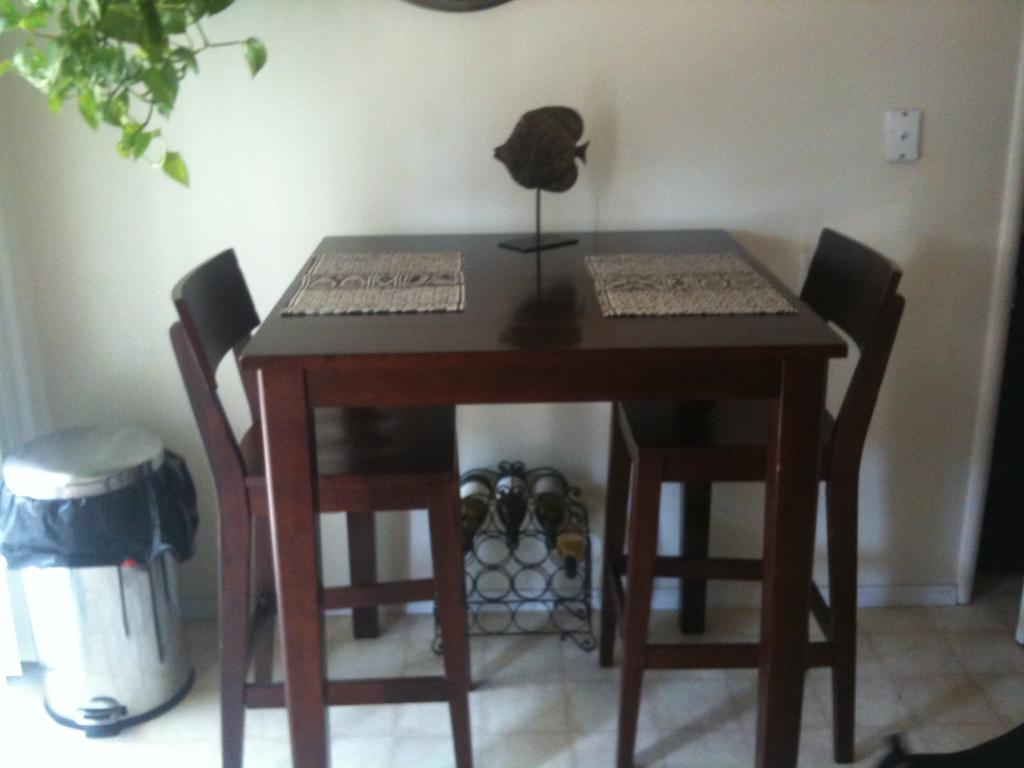
\includegraphics[width=.4\textwidth]{/Users/apple/OVGU/Thesis/code/3dReconstruction/report/images/pix3d/pix3d_5}}\quad
    \subfloat[][]{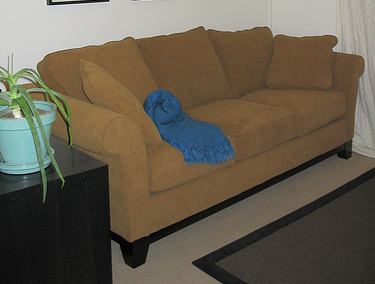
\includegraphics[width=.4\textwidth]{/Users/apple/OVGU/Thesis/code/3dReconstruction/report/images/pix3d/pix3d_2}}\\
    \subfloat[][]{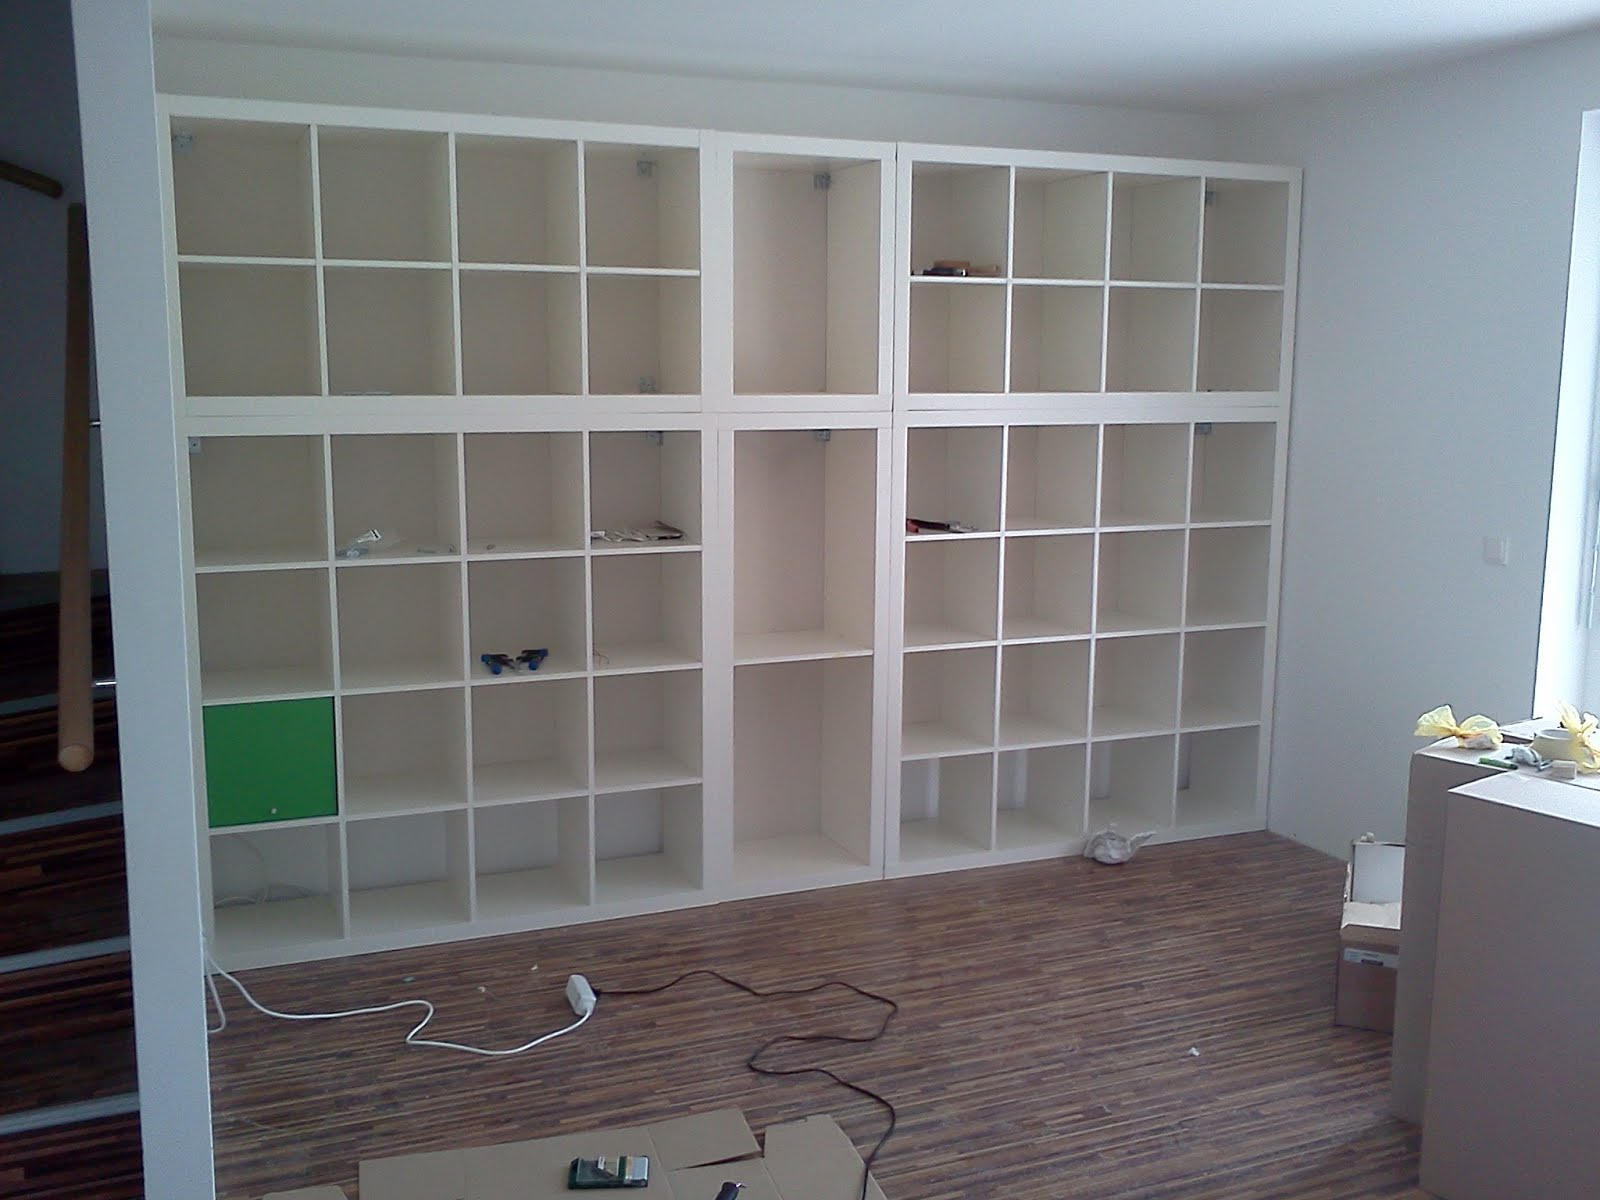
\includegraphics[width=.4\textwidth]{/Users/apple/OVGU/Thesis/code/3dReconstruction/report/images/pix3d/pix3d_6}}\quad
    \subfloat[][]{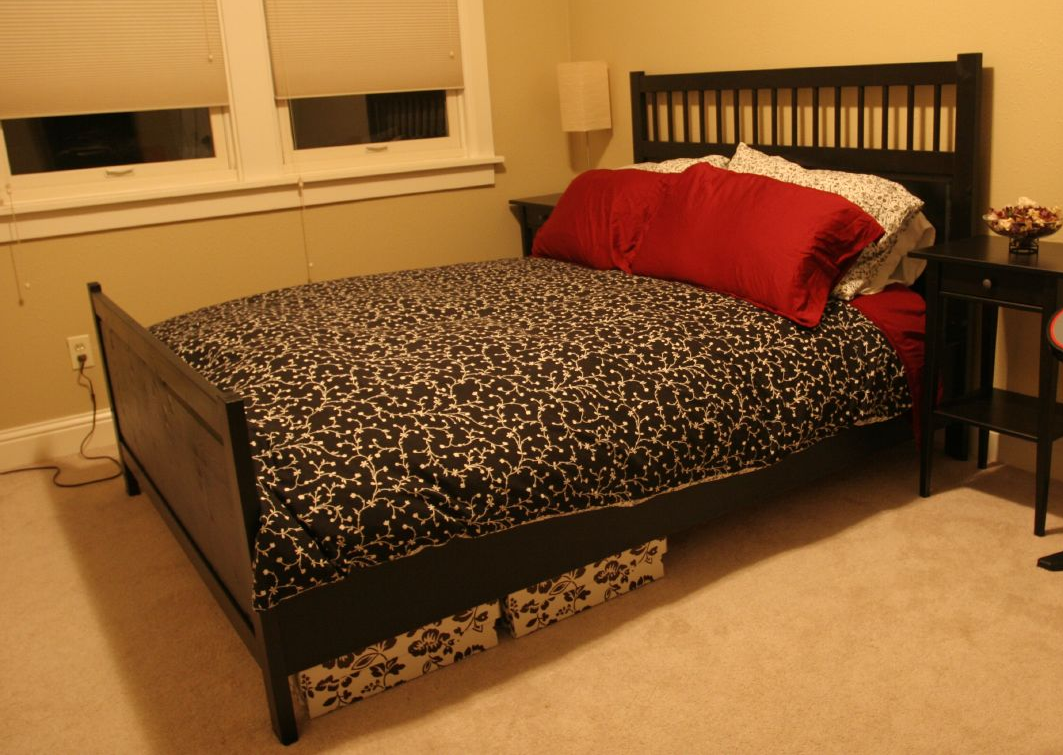
\includegraphics[width=.4\textwidth]{/Users/apple/OVGU/Thesis/code/3dReconstruction/report/images/pix3d/pix3d_4}}
    \caption{Sample RGB images from pix3D}
    \label{fig:Pix3D samples}
\end{figure}

\section{Role of SceneNet}\label{sec:role-of-scenenet}
SceneNet~\cite{McCormac:etal:ICCV2017} is an extensive collection of photorealistic indoor scene trajectories.
The dataset provides images and videos of indoor scenes that can be used for tasks like SLAM,
semantic and instance segmentation, object detection, and further enhanced for other vision problems like optical flow depth and pose estimation ~\cite{McCormac:etal:ICCV2017}).
They use ShapeNet~\cite{chang2015shapenet} models to occupy 57 indoor scenes, giving the scene unlimited configurations.
Unfortunately, there is no mapping from scene to 3D model for tasks like 3D reconstructions.
In our approach, we utilize the scene provided by SceneNet as a layout for our indoor scenes.
Each scene includes initial Shapenet models with furniture placement.
We then replace the class under observation with a corresponding model from Pix3D.

\section{Unity-based pipeline}\label{sec:unity-based-pipeline}
To create the synthetic dataset, we use Unity Game Engine.
The reasons for selecting Unity as our platform for the application are:
\begin{enumerate}
    \item Cross-platform game engine and hence usable on any Operating system.
    \item The basic version is available for free.
    \item Provides all the necessary tools to create an ersatz environment with well-maintained documentation.
    \item An active developer community.
\end{enumerate}

There is no official comparison between Unreal Engine and Unity engine to have a deciding factor.
The selection of the Unity engine was a purely individual choice and ease of use.
However, both these game engines can create realistic-looking scenes that are usable for synthetic dataset generation.
With the Unity game engine, the available scenes from the Scenenet and 3D models from Pix3D can be imported to form an ersatz environment.
Further domain randomization can be applied to create a dataset of photorealistic images and 2.5D data like normals, depth maps, masks.

\subsection{Domain Randomization with Unity Engine}\label{subsec:domain-randomisation-with-unity-engine}
In this section, we discuss what kind of domain randomization we apply for dataset creation.

\subsubsection{Scenes from SceneNet}\label{subsubsec:scenes-from-scenenet}
As discussed in \autoref{sec:role-of-scenenet}, SceneNet provides a wide variety of indoor scenes, including bedrooms, bathrooms, living rooms, kitchens, and offices.
We did not consider the bathroom for our case, as the categories under observations are furniture which we rarely see in the bathroom.
For the rest of the scenes, we have a pre-determined setup given by SceneNet.
We use 25 scenes in total as basic rooms to insert our target object.
Moreover, we feel this should be sufficient to check if Unity can produce a helpful dataset with further randomization.

\subsubsection{Camera Viewpoints}
The position and orientation of the camera give us the most randomization in this setup.
The user can choose the minimum and maximum distance to place the camera from the target object.
A random point is selected in this range as the position for the camera.
The camera is oriented such that it always looks at the target object, irrespective of its position.
With this, we achieved different backgrounds for the target object, and the target object appears to be indifferent positions and orientations.

\subsubsection{Lighting and shadows}
Lighting plays a vital role in photorealism.
If the lighting is not set up correctly, the synthetic dataset will never seem to be photorealistic.
Unity offers a wide variety of lighting like global light, which acts like sunlight, and various indoor lighting systems.
Ideally, we should make the luminous objects like lamps, chandeliers, bulbs, etc.,
the source of light for indoor scenes, but we observed that the room does not light up uniformly,
making it less photorealistic.
Hence we use some pre-determined lighting settings, discussed further in implementation(\autoref{sec:3d-scene-framework}).

\subsubsection{Randomized textures}
SceneNet~\cite{McCormac:etal:ICCV2017} also provide textures for different categories in the scene.
We further increase the texture database by adding more textures from ambientCG.com, which provides free licenses.
We randomly allocate textures to each object, ensuring that each category has the same texture to make the scene more uniform.

\subsubsection{Replacing target objects}
To further randomize the scene, the category of target objects is replaced by the object under observation.
When more than one object of the same category is present, we randomize the object to be replaced, further randomizing the captured data.
The target object is scaled such that the least dimension of the target object matches the least dimension of the category object in the scene.
For example, if the length of the category object in the scene is the most petite amount length, width, and height, then the target object is scaled to match this length.
The rescaling makes the target object blend in with the scene.

\section{\gls{free}, a Pix3D based synthetic dataset}\label{sec:s2r:3d-free-a-pix3d-based-synthetic-dataset}

\gls{free} dataset, which stands for Synth2Real: 3-Dimensional Furniture Reconstruction from Ersatz Environment, combines SceneNet and Pix3D dataset.
We utilize the availability of 3D models of rooms and pieces of furniture from these two datasets to create an ersatz environment using Unity as our framework.
We randomize the indoor scenes from SceneNet~\cite{McCormac:etal:ICCV2017} and textures provided by them with some additional complex textures.
The other option would have been to use the ShapeNet as the target model, but we would not have a real dataset to compare to this case.
Ideally, a model trained on ShapeNet should also perform well with a real dataset like Pix3D, but we decided to have a synthetic dataset based on Pix3D itself for better comparison.

\section{3D reconstruction pipeline}\label{sec:3D reconstruction pipeline}
We create a pipeline for processing the 3D reconstruction task.
The backbone of the pipeline is the base model and the dataset being used to train.
In this section, we discuss the model used as a base and the rationale behind its selection.

\subsection{Pix2Vox and Pix2Vox++}\label{subsec:pix2vox-and-pix2vox++}
The architecture of pix2vox~\cite{Xie_2019} is as shown in \autoref{fig:architectures}(a).
The network consists of 4 modules: Encoder, Decoder, Merger, and Refiner.
Merger plays a significant part when it comes to the multi-view reconstruction of 3d objects.
As we focus on single-view 3d reconstruction, the merger module will not influence the output significantly.
As an encoder, pix2vox has utilized \gls{vgg}16 network~\cite{simonyan2015deep} pre-trained on ImageNet~\cite{Deng2009ImageNetAL}.
The decoder is an expansive network that converts 2D embeddings to a 3D voxel grid.
The refiner is an auto-encoder that takes the 3D output from the merger and produces a more refined final output.
A second paper based on pix2vox was titled Pix2Vox++~\cite{Xie_2020}.
The extended work replaces \gls{vgg} encoder~\cite{simonyan2015deep} with \gls{resnet}~\cite{He2016DeepRL}.


\begin{figure}[!ht]
    \centering
    \subfloat[][]{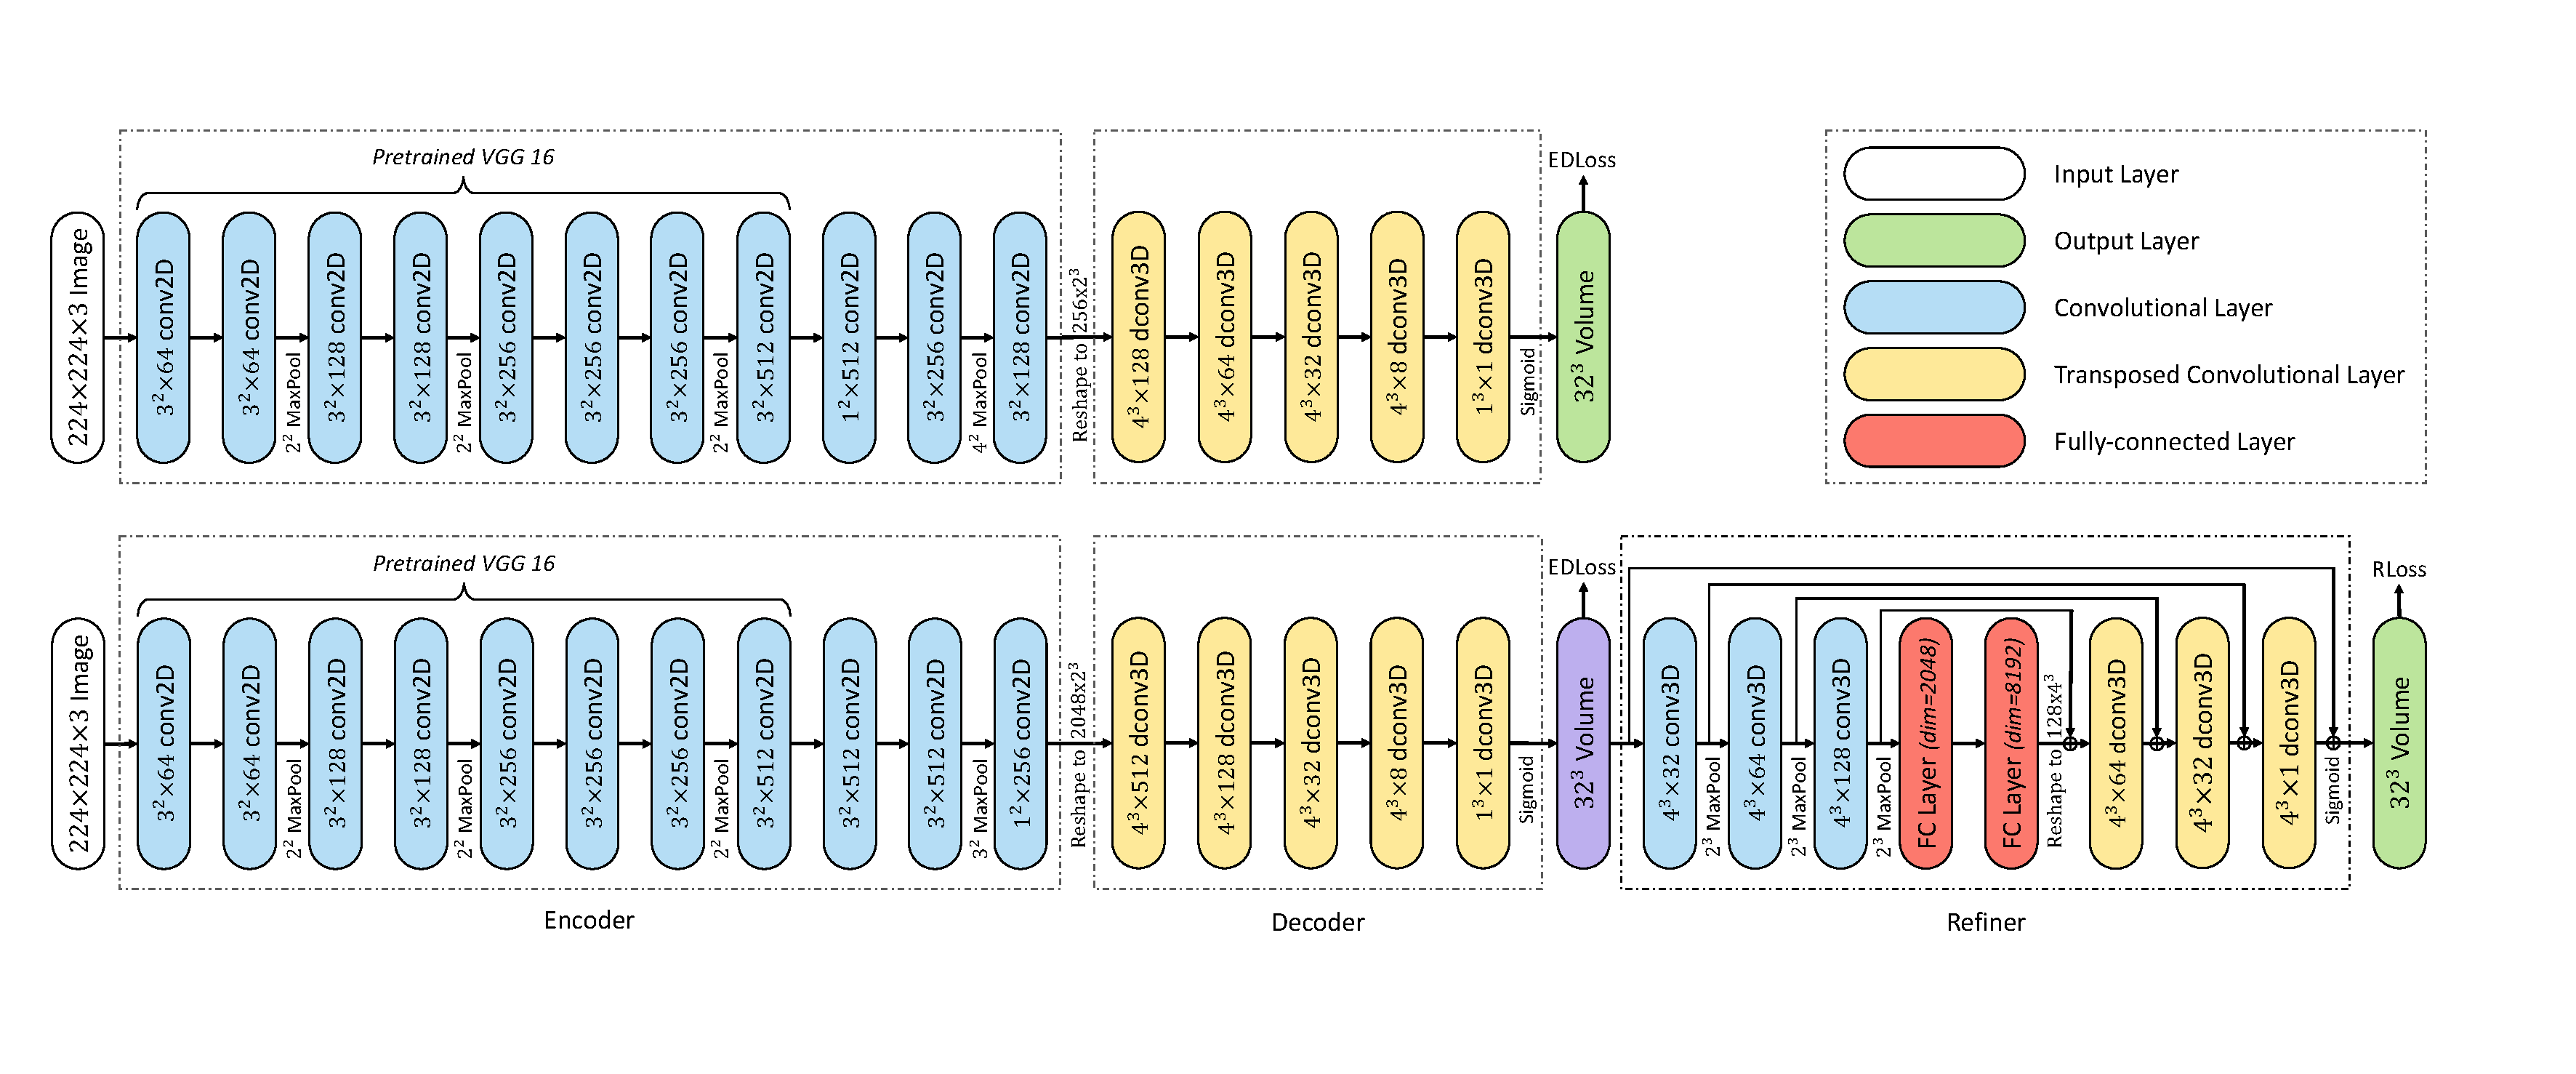
\includegraphics[angle=-90,width=0.45\linewidth]{/Users/apple/OVGU/Thesis/code/3dReconstruction/report/images/concept/pix2vox}}\quad
    \subfloat[][]{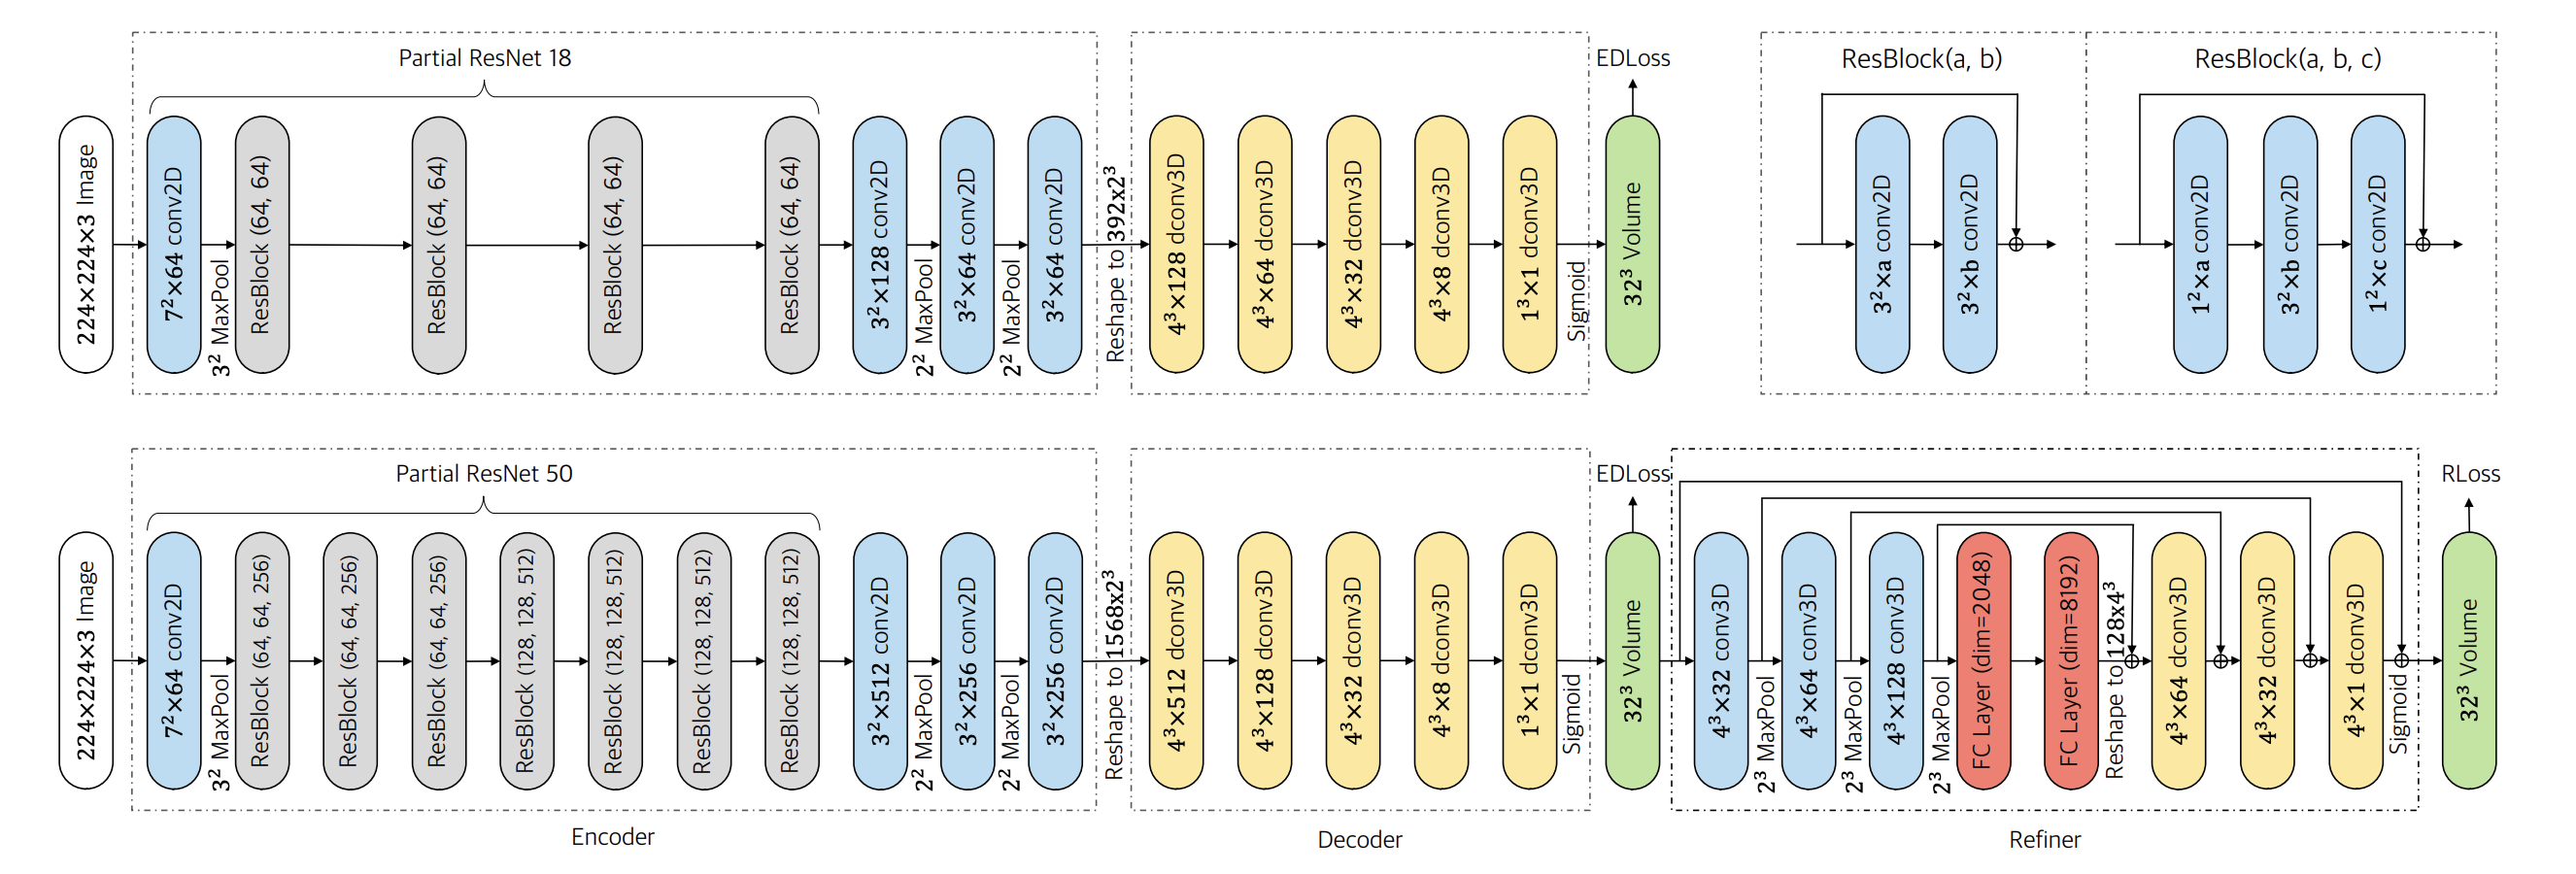
\includegraphics[angle=-90,width=0.45\linewidth]{/Users/apple/OVGU/Thesis/code/3dReconstruction/report/images/concept/pix2voxpp}}\\
    \caption{Network architectures used as a baselines (a)Pix2Vox (b)Pix2Vox++}
    \label{fig:architectures}
\end{figure}

\subsection{Why Pix2Vox?}\label{subsec:why-pix2vox?}
Pix2Vox has been used as a baseline by most of the research-oriented to 3D reconstruction.
This network is one of the few networks to be tested on the Pix3D dataset.
According to the survey conducted by~\cite{Han2021ImageBased3O}, the performance of pix2vox~\cite{Xie_2019}
is significantly higher compared to previous work(\cite{DBLP:journals/corr/TulsianiZEM17,tatarchenko2016multiview,richter2018matryoshka,gwak2017weakly,8265323}), as shown in \autoref{fig:survey on 3d reconstruction}.
At the same time, this comparison was made on 3d reconstruction of the ShapeNet dataset since Pix3D was not available when previous work was published.
From our survey, only CoReNet~\cite{popov2020corenet} had a slight gain in performance compared to pix2vox.
When trained on ShapeNet and tested with Pix3D, CoReNet gave a result of 29.7\% \gls{iou} while Pix2Vox gave a result of 28.8\% \gls{iou}  and Pix2Vox++ a result of 29.2\% \gls{iou}\@.
Since the difference in the performance was not significant, we decided to stick with the baseline model.
Another reason for selecting the pix2vox model is that the backbone of the architecture is pre-trained with ImageNet.
Hence, the embeddings generated from this encoder can help visualize the domain space of both Pix3D (real images)  and \gls{free}(synthetic images).
As mentioned above, for pix2vox++, the \gls{resnet} is the backbone encoder with 25\% lesser parameters and 5\% lesser inference time than \gls{vgg}\@.
In addition, the author even demonstrated that Pix2vox++ performs 1.5\% better than pix2vox.
The architecture of pix2vox++ is as shown in \autoref{fig:architectures}(b).
Furthermore, the focus of this thesis is not to check which is the best model to reconstruct the furnitures, but to check if game engines can produce photorealistic images usable for 3d reconstruction.
Hence the selection of the model was not of utmost importance.
However, since the two architectures are relatable, it would be interesting to compare the results for the 3D Reconstruction task.

%\begin{figure}
%    \centering
%    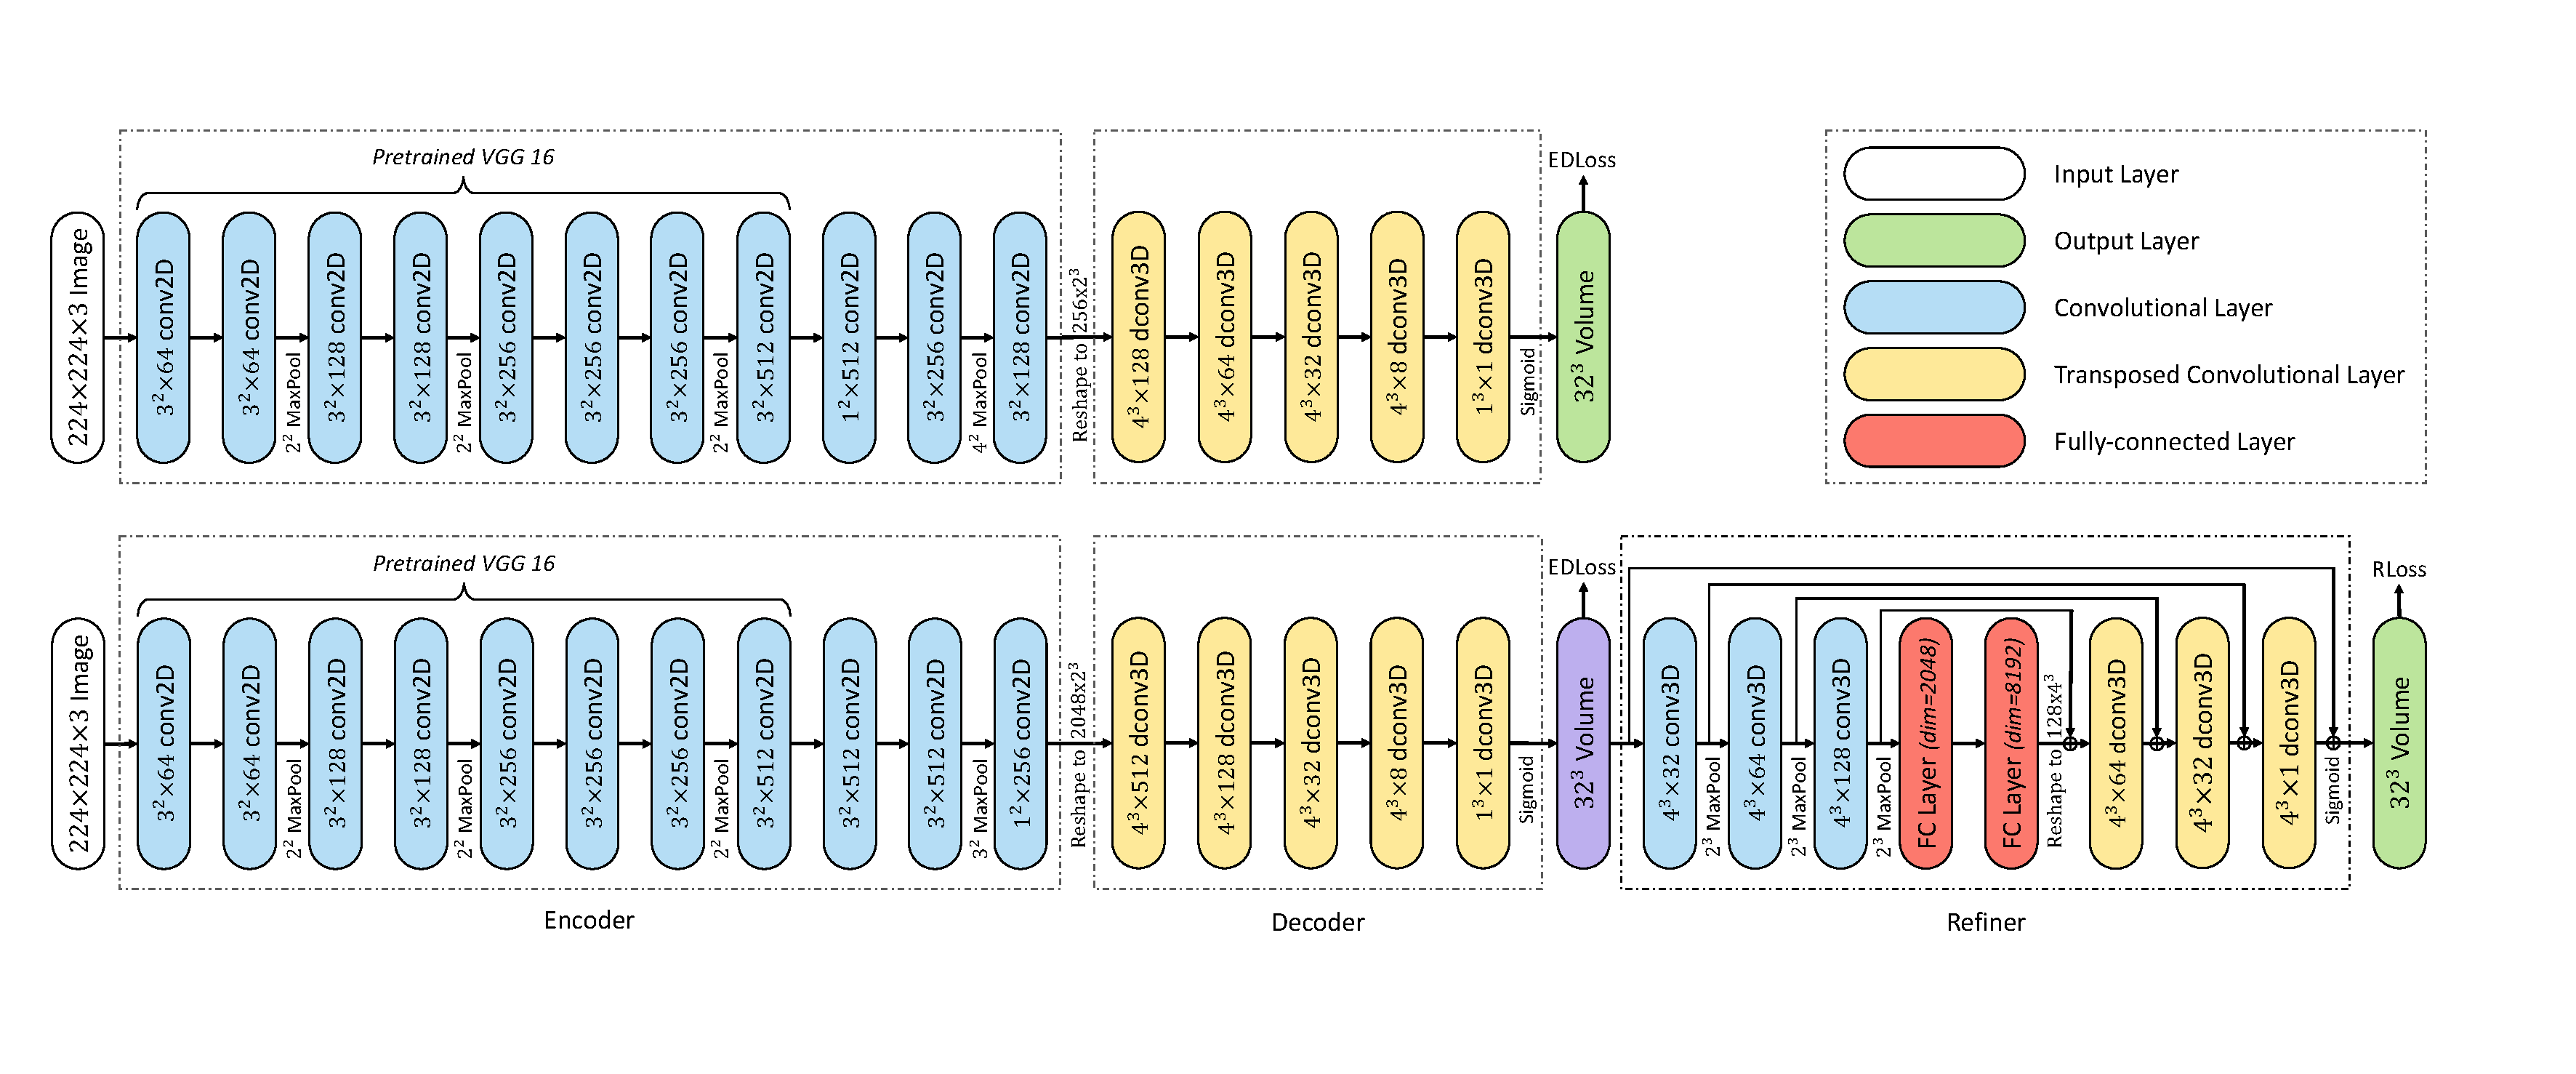
\includegraphics[width=\textwidth]{/Users/apple/OVGU/Thesis/code/3dReconstruction/report/images/concept/pix2vox}
%    \caption{Network architecture for pix2vox~\cite{Xie_2019}}
%    \label{fig:pix2vox architecture}
%\end{figure}
%
%\begin{figure}
%    \centering
%    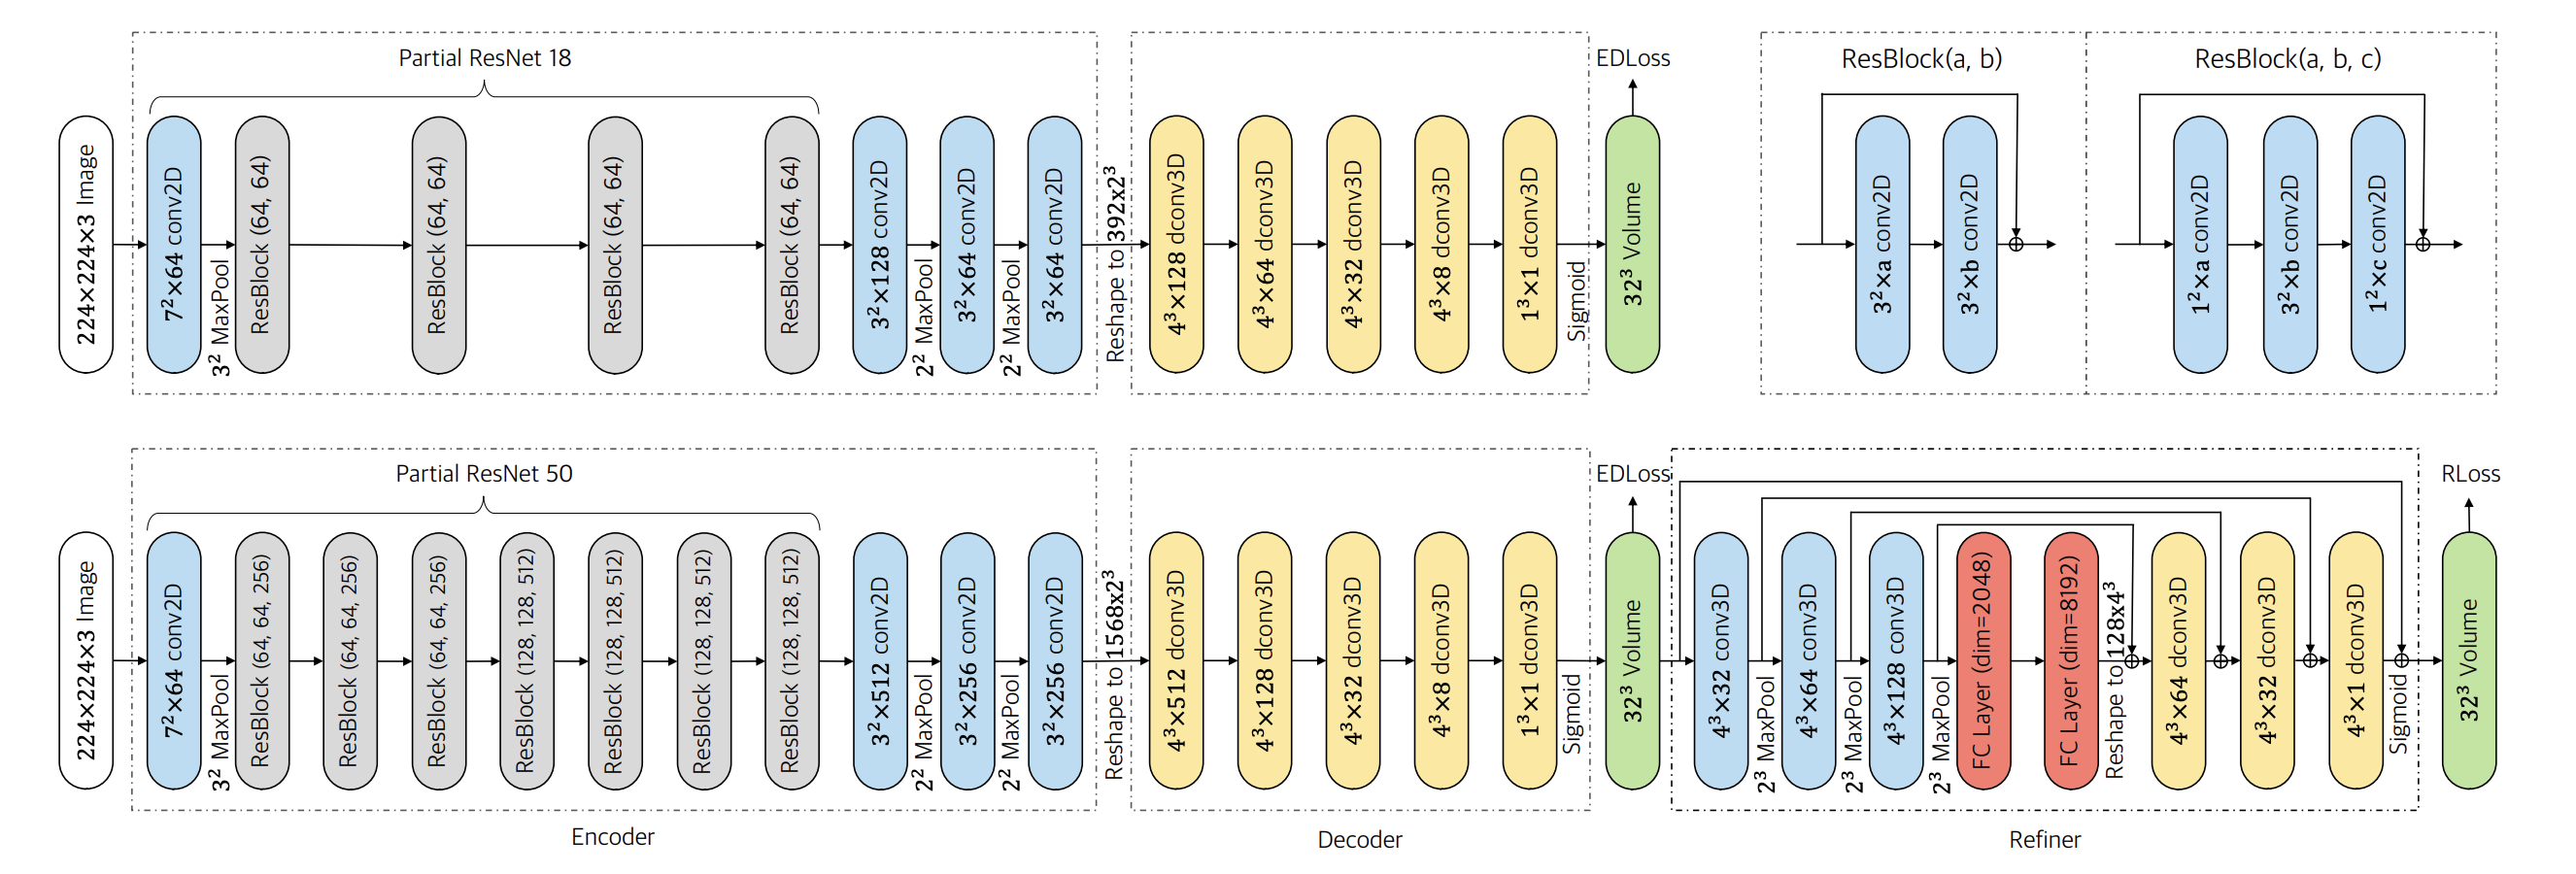
\includegraphics[width=\textwidth]{/Users/apple/OVGU/Thesis/code/3dReconstruction/report/images/concept/pix2voxpp}
%    \caption{Network architecture for pix2vox++~\cite{Xie_2020}}
%    \label{fig:pix2voxpp architecture}
%\end{figure}

\begin{figure}[ht]
    \centering
    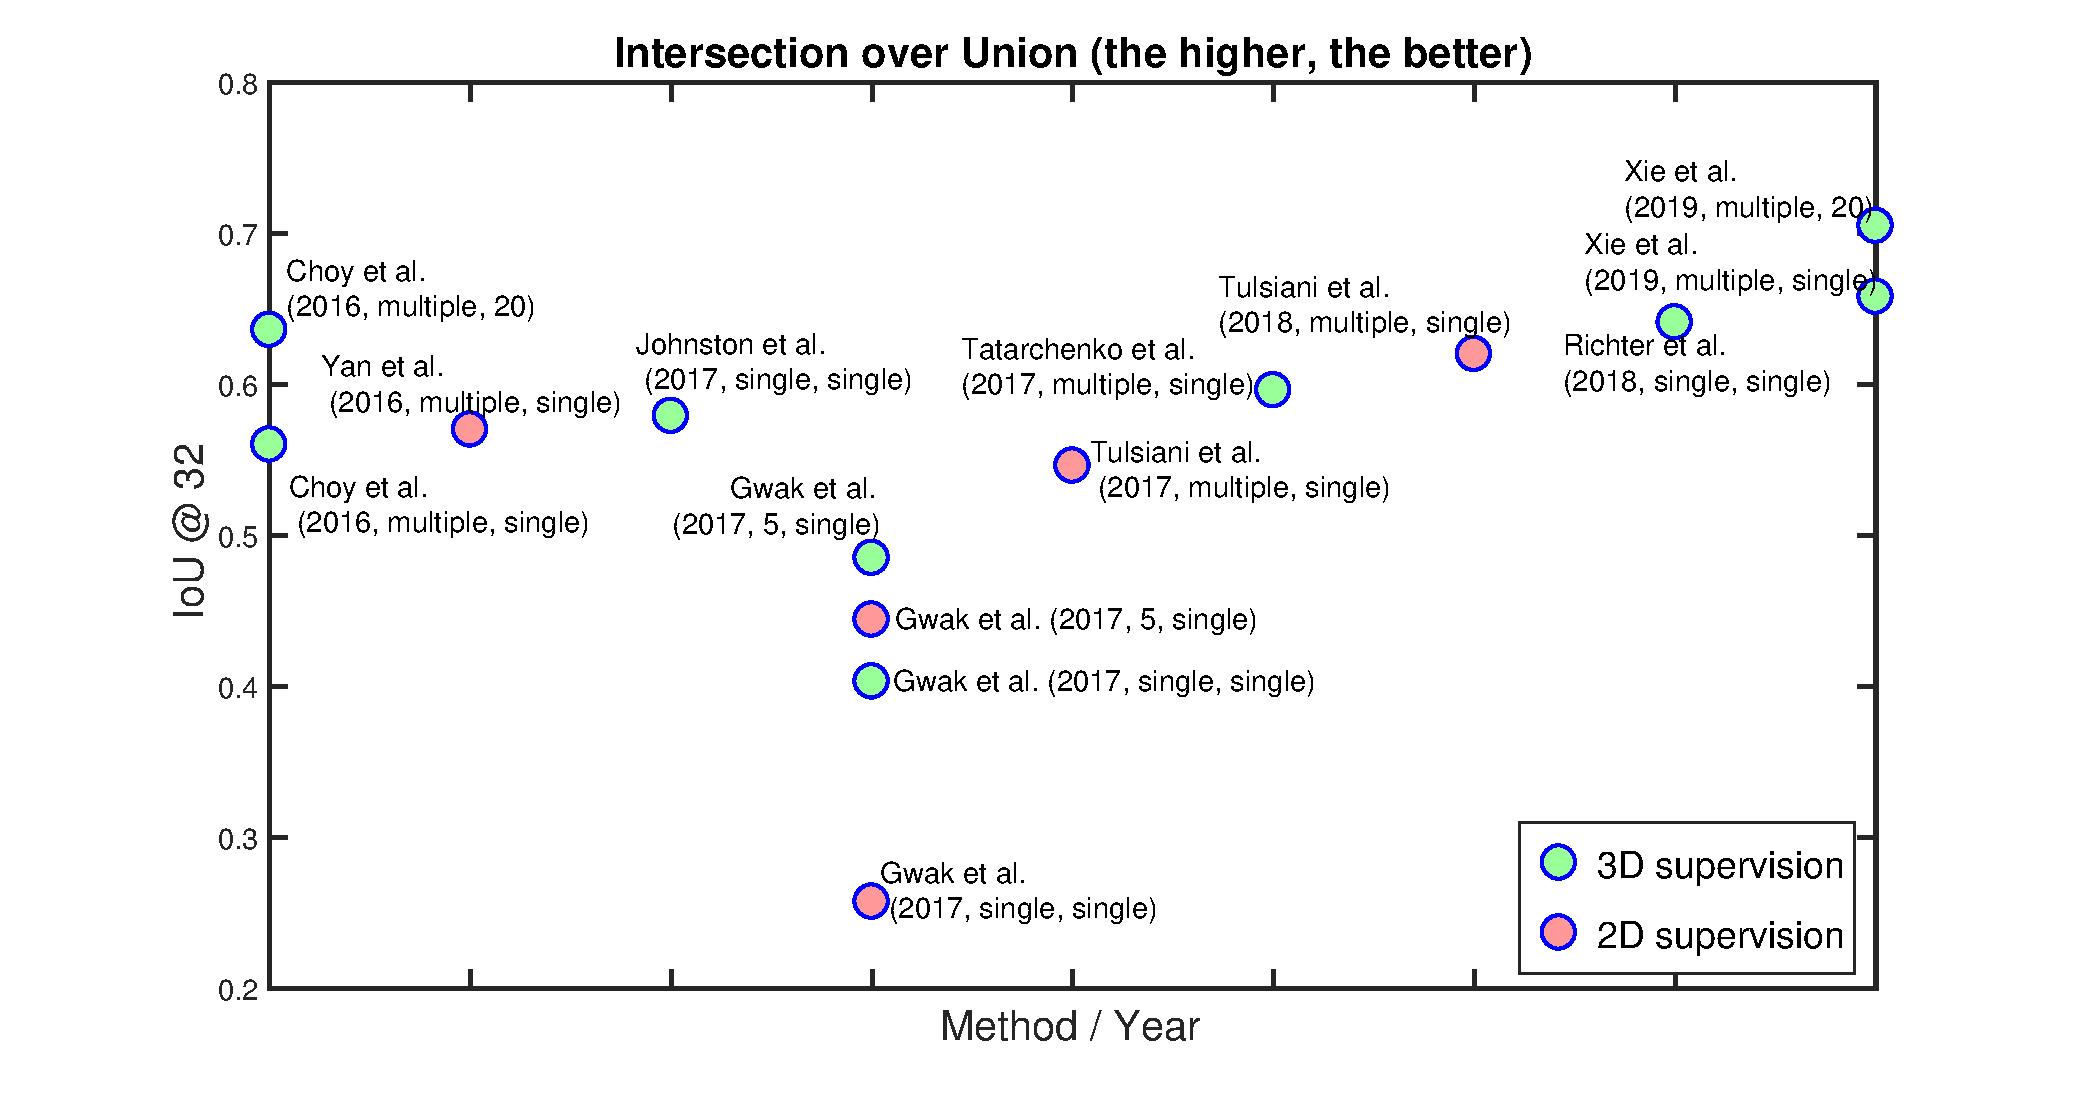
\includegraphics[width=\textwidth]{/Users/apple/OVGU/Thesis/code/3dReconstruction/report/images/concept/survey}
    \caption{A survey conducted by~\cite{Han2021ImageBased3O}, demonstrates that Pix2Vox is considerably a good 3D reconstruction model.
    The values are from 3D reconstruction of ShapeNet~\cite{chang2015shapenet} since Pix3D was not published by then.}
    \label{fig:survey on 3d reconstruction}
\end{figure}

%\section{Domain adaptation with Gan \todo{if we decide to go with this approach}}

\section{Domain space}\label{sec:domain-space}

Since this thesis includes image datasets from different domains, it is essential to understand the domain space of these datasets.
This section discusses how we intend to visualize the domain space and a quantitative measure to indicate the difference between the domains.

\subsection{Visualizing with \gls{tsne}}\label{subsec:visualizing-with-tsne}
\gls{tsne} stands for t-Distributed Stochastic Neighbor Embedding~\cite{vanDerMaaten2008}; it is a tool to visualize a high dimensional space in a low dimension space while retaining the information of high dimension as much as possible.
In our case, the images are embedded using a \gls{vgg}16 network with an output dimension of 1000.
This multi-dimensional output is converted to two-dimension for better visualization of the embedding space.

In this segment, we briefly explain how \gls{tsne} works.

\begin{enumerate}
    \item \textbf{Step 1}: Calculate the similarity between points in high dimensional space using a joint probability distribution.
        To achieve this, the Euclidean distances between each point is transformed into conditional probability distribution as in \autoref{eq:equation1}, which represents similarity between a pair of points.
        The conditional probability of a point $x_i$ with point $x_j$ to be located next to it, is represented by a Gaussian with center at $x_i$.
        Normalising is done to handle the different cluster densities.
        Conditional probability is converted to Joint probability using \autoref{eq:equation2}.
    \begin{equation}
        p_{j \mid i}=\frac{\exp \left(-\left\|x_{i}-x_{j}\right\|^{2} / 2 \sigma_{i}^{2}\right)}{\sum_{k \neq i} \exp \left(-\left\|x_{i}-x_{k}\right\|^{2} / 2 \sigma_{i}^{2}\right)}
        \label{eq:equation1}
    \end{equation}

    \begin{equation}
        p_{i j}=\frac{p_{j \mid i}+p_{i \mid j}}{2 n}
        \label{eq:equation2}
    \end{equation}

    \item \textbf{Step 2}: Using a random point dataset on a lower dimension with same number of points in higher dimension, a Joint probability distribution is created but with a Student-t distribution instead of Gaussian.
    This is represented by \autoref{eq:equation3}.
    t-distribution makes sure that the projection in low dimension is not concentrated on a single point.
    \begin{equation}
        q_{ij} = \frac{(1+\left \| y_{i}-y_{j} \right \|^{2})^{-1}}{\sum _{k\neq l} (1+\left \| y_{k}-y_{l} \right \|^{2})^{-1}}
        \label{eq:equation3}
    \end{equation}

    \item \textbf{Step 3}: Learn to represent the high dimension space in low dimension by making the Joint distribution of the lower dimension as close as possible to that of the higher dimension.
    For this Kullback-Leiber divergence\cite{Joyce2011} is used to compare the similarity between the two distributions as in \autoref{eq:equation4}.
    Using gradient descent, the cost function based on KL-divergence (\autoref{eq:equation5}) is minimized to make the points fall in place.

    \begin{equation}
        D_{\mathrm{KL}}(P \| Q)=\sum_{x \in \mathcal{X}} P(x) \log \left(\frac{P(x)}{Q(x)}\right)
        \label{eq:equation4}
    \end{equation}

    \begin{equation}
        C=K L(P \| Q)=\sum_{i} \sum_{j} p_{i j} \log \frac{p_{i j}}{q_{i j}}
        \label{eq:equation5}
    \end{equation}
\end{enumerate}

Perplexity is a parameter that informs the algorithm on how much attention to give the local and global features.
The publication~\cite{vanDerMaaten2008} indicates the values between 5 and 50 to be a good initialization.
An article on \gls{tsne} interpretation~\cite{wattenberg2016how} informs us to have a perplexity value lesser than the total number of points.
    It also notes that the cluster distance may not be as the intuition suggests, i.e., greater distance may not necessarily mean good separation, or lesser distance does not inevitably mean closer similarity for well-separated clusters.
    However, \gls{tsne} can still visualize if the clusters are overlapping or have a shared embedding space or not.
    Hence, we will use \gls{tsne} as a medium to visualize the embedding space without giving importance to the distance or the scale of the plots.

%\subsection{Maximum Mean Discrepancy(MMD)}
\subsection{Fr\'echet Inception Distance(FID))}\label{subsec:fr'echet-inception-distance)}
For quantitative measure, we use \gls{fid}
\gls{fid} \cite{Heusel2017GANsTB} was specifically formulated to evaluate the performance of Generative Adversarial Networks \cite{Goodfellow2014GenerativeAN}.
The core idea behind \gls{fid} was to evaluate the generated synthetic images using the statistics collected from both synthetic and real images.
Lower the value of \gls{fid} better the quality of the images.

The embeddings of the images are calculated by passing it through an Inception v3 model~\cite{Szegedy2016RethinkingTI} pre-trained on ImageNet~\cite{Deng2009ImageNetAL}.
The output layer is removed, and the penultimate pooling layer activations are used to get the embedding vector.
This vector has a dimension of 2048.
The images from both synthetic and real datasets are passed through the model, and the obtained statistics is used to calculated the \gls{fid} as in \autoref{eq:fid}.

\begin{equation}
    d^{2}\left((\boldsymbol{\mu}_{r}, \boldsymbol{C}_{r}),\left(\boldsymbol{\mu}_{s}, \boldsymbol{C}_{s}\right)\right)=\left\|\boldsymbol{\mu}_{r}-\boldsymbol{\mu}_{s}\right\|^{2}+\operatorname{Tr}\left(\boldsymbol{C}_{r}+\boldsymbol{C}_{s}-2\left(\boldsymbol{C}_{w} {C}_{w}\right)^{1 / 2}\right)
    \label{eq:fid}
\end{equation}

In the above \autoref{eq:fid}, $\mu_r$ and $\mu_s$ are feature-wise mean for real and synthetic images, $C_r$ and $C_s$ are respective covariance matrices.
$Tr$ is the Trace linear algebra operation, which is the sum of main diagonal elements.



